\section{Experiments}\label{section:experiments}
In this section, we present the experimental evaluation of LMFormer. We first describe the datasets and experimental setup, followed by a detailed quantitative and qualitative performance analysis. Our goal is to demonstrate the effectiveness of LMFormer on both standard benchmarks and real-world-inspired scenarios while also highlighting its generalization ability across different datasets.

\subsection{Experimental Setup}\label{subsection:exp_setup}
\textbf{Dataset:} As we aim to evaluate LMFormer’s performance in structured urban environments as well as more diverse intersection-heavy scenarios, we selected the nuScenes \cite{caesar2020nuscenes} and the Deep Scenario \cite{lu2023deepscenario} datasets for benchmarking. The nuScenes dataset comprises driving scenarios from Boston and Singapore, generated using sensor data of a moving vehicle in complex scenarios. The Deep Scenario dataset is built from recordings of stationary drones, placed vertically above complex traffic scenarios, e.g. intersections.

\noindent\textbf{Metrics:} We report the quantitative performance of LMFormer on the nuScenes and Deep Scenario datasets in terms of minADE\textsubscript{k}, minFDE\textsubscript{k}, MR\textsubscript{k}, and OffRoadRate. minADE\textsubscript{k} measures the average Euclidean distance between the ground truth and the best-matching trajectory among the top-$k$ predicted trajectories. A lower value indicates better alignment with the actual observed path. This metric is particularly relevant for multi-modal prediction settings, where multiple future outcomes are possible. minFDE\textsubscript{k} computes Euclidean distances between the endpoint of the ground truth and the best prediction among the top-$k$ trajectories. It indicates how well the network predicts the final goal position. MR\textsubscript{k} measures the fraction of misses, where a miss occurs when the maximum pointwise $L_2$ distance between the ground truth and predicted trajectories is larger than two meters. A small value indicates that the predicted velocity profile matches the ground truth well. Finally, the OffRoadRate metric reports the fraction of predicted trajectories outside the drivable area.

\noindent\textbf{Implementation Details:} We train LMFormer on one Nvidia A100 GPU using AdamW Optimizer \cite{loshchilov2018decoupled}. As required by nuScenes Prediction Challenge \cite{nuscene2020prediction}, the duration of the input trajectory is limited to 2 seconds and that of the output trajectory to 6 seconds, with a sampling rate of 2Hz.  Also, the maximum number of modes $k$ is set to 5, to compute minADE\textsubscript{5} and MR\textsubscript{5} for the comparison against other SOTA methods. The same configurations are extended to the Deep Scenario Dataset, as it does not specify any restrictions on the aforementioned hyperparameters. 

Both static and dynamic contexts enclose an area of 150m x 100m, where the former is along the driving direction. In order to help the model generalize for both left-hand and right-hand driving conditions, the inputs are flipped along the driving direction with a probability of 50\%. We also identify that increasing the number of stacked layers $N$ beyond 3 does not improve the network performance, and hence we set $N$ = 3 to keep the computational costs to a minimum. A similar observation is made for the length of a lane segment, and its optimum value is recorded at 3 meters. 

\subsection{Results and Discussion}\label{subsection:results}
\begin{table}[b]
    \centering
    \caption{Comparison with state-of-the-art on the nuScenes prediction challenge test split.}
    \label{tab:experiment_table}
    \resizebox{\linewidth}{!}{
    \begin{tabular}{l|c c|c|c}
    \hline
    Method & minADE\textsubscript{5}$\downarrow$ & MR\textsubscript{5}$\downarrow$ & minFDE\textsubscript{1}$\downarrow$ & OffRoad$\downarrow$ \\
    \hline
    GOHOME \cite{gilles2022gohome}  & 1.42 & 0.57 & 6.99 & 0.04 \\
    Autobot \cite{girgis2021latent}  & 1.37 & 0.62 & 8.19 & 0.02 \\
    THOMAS \cite{gilles2022thomas}  & 1.33 & 0.55 & 6.71 & 0.03 \\
    PGP \cite{deo2021multimodal}  & 1.27 & 0.52 & 7.17 & 0.03 \\
    MacFormer \cite{feng2023macformer}  & 1.21 & 0.57 & 7.50 & 0.02 \\
    LAFormer \cite{liu2024laformer}  & 1.19 & 0.48 & 6.95 & 0.02 \\
    Socialea \cite{chen2023q} & 1.18 & 0.48 & 6.77 & 0.03 \\
    FRM \cite{park2023leveraging}  & 1.18 & 0.48 & 6.59 & 0.02 \\
    CASPNet\_v2 \cite{schafer2023caspnet++} & 1.16 & 0.50  & \textbf{6.18} & \textbf{0.01} \\
    CASPFormer \cite{yadav2025caspformer} & 1.15 & 0.48 & 6.70 & \textbf{0.01} \\
    SemanticFormerR \cite{sun2024semanticformer} & \textbf{1.14} & 0.50 & 6.27 & 0.03 \\
    \hline
    LMFormer (ours) & \textbf{1.14} & \textbf{0.47} & 6.85 & \textbf{0.01} \\
    \hline
    \end{tabular}
    }
\end{table}

We provide a comparison of LMFormer against the SOTA networks on the nuScenes Motion Prediction Challenge test split \cite{nuscene2020prediction} in Table \ref{tab:experiment_table}. LMFormer achieves SOTA results across minADE\textsubscript{5}, MR\textsubscript{5} and OffRoadRate. Qualitative results are depicted in Figure \ref{fig:nuScenes_qual}. As is evident, the trajectories undergo a substantial enhancement during the refinement process. It is noteworthy that the network is capable of making diverse predictions and aligning the predicted trajectories with a high degree of accuracy with the lanes. Furthermore, the attention map provides insight into the underlying learning behaviors of LMFormer. We observe that the network pays higher attention to the lanes, which are important for predicting its future trajectory.

It is important to note that despite achieving SOTA performance across all other metrics, LMFormer does not achieve SOTA on minFDE\textsubscript{1}. We suspect that this behavior emerges due to the fact that the predicted trajectories have to align with the lanes, which is rarely the case in the real world. Such lane alignment would predominantly impact the predicted position towards the end of the trajectory compared to the initial ones. Thus, the results of this effect are more pronounced in minFDE\textsubscript{k} compared to minADE\textsubscript{k} and MR\textsubscript{k}.

We additionally investigate the worst reported prediction of LMFormer based on the minADE\textsubscript{5} metric (see Figure \ref{fig:nuScenes_worst}). Interestingly, even though the network generates diverse predictions, the predicted velocity for the mode following the ground truth path can be suboptimal, resulting in a bad minADE\textsubscript{k}. Thus, we hypothesize that the performance of the motion prediction modules can be improved by separately predicting velocity profiles and future paths. The work by Sun et al. \cite{sun2024semanticformer} also reports a similar observation, i.e., if the prediction modules have access to the ground truth velocity, the performance of the models improves significantly. Given this evidence, the direction of separation between velocity and path prediction should be explored in future work. 

\begin{figure}
    \centering
    \begin{subfigure}[t]{0.4\linewidth}
        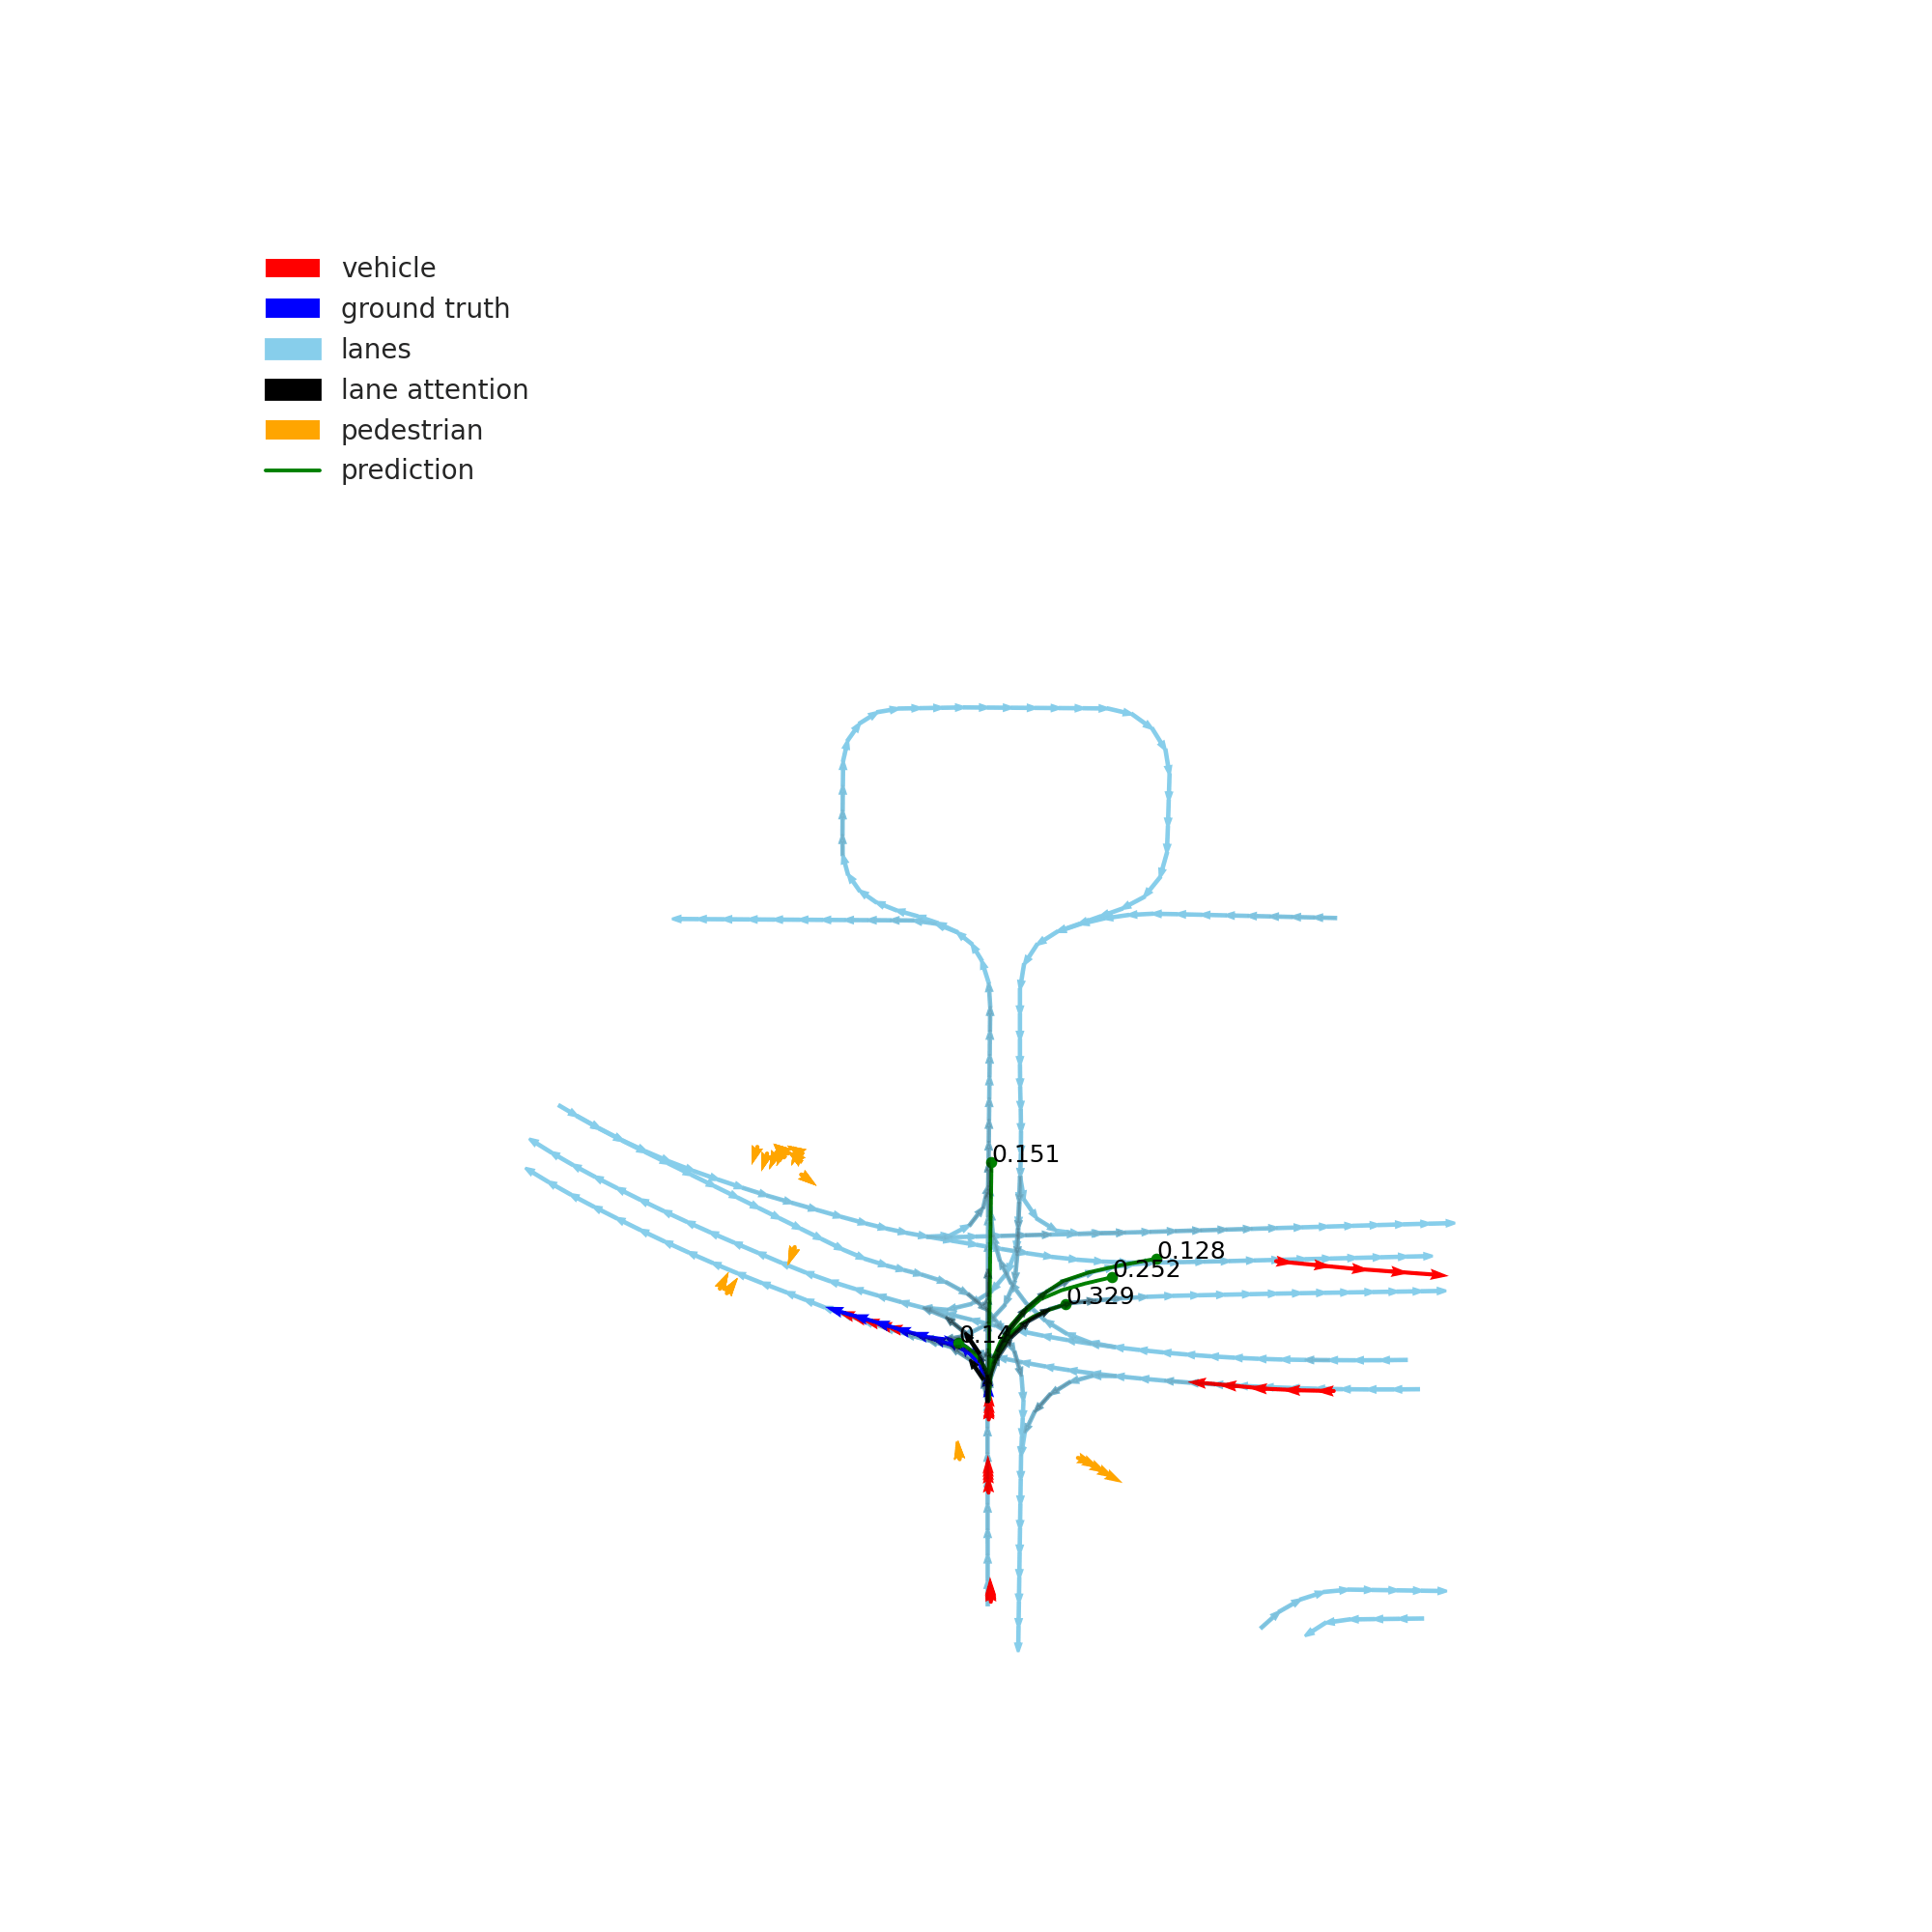
\includegraphics[height=4cm,trim={300 140 260 360},clip]{images_results/4b432f819ef44455882cb2e4d5d375ef_4809652b5d2a4ea29bbe1bbb1bacd43a_minADE5_5.72_2-min.png}
        % \caption{Final Trajectories}
    \end{subfigure}
    % \begin{subfigure}[t]{0.4\linewidth}
    %     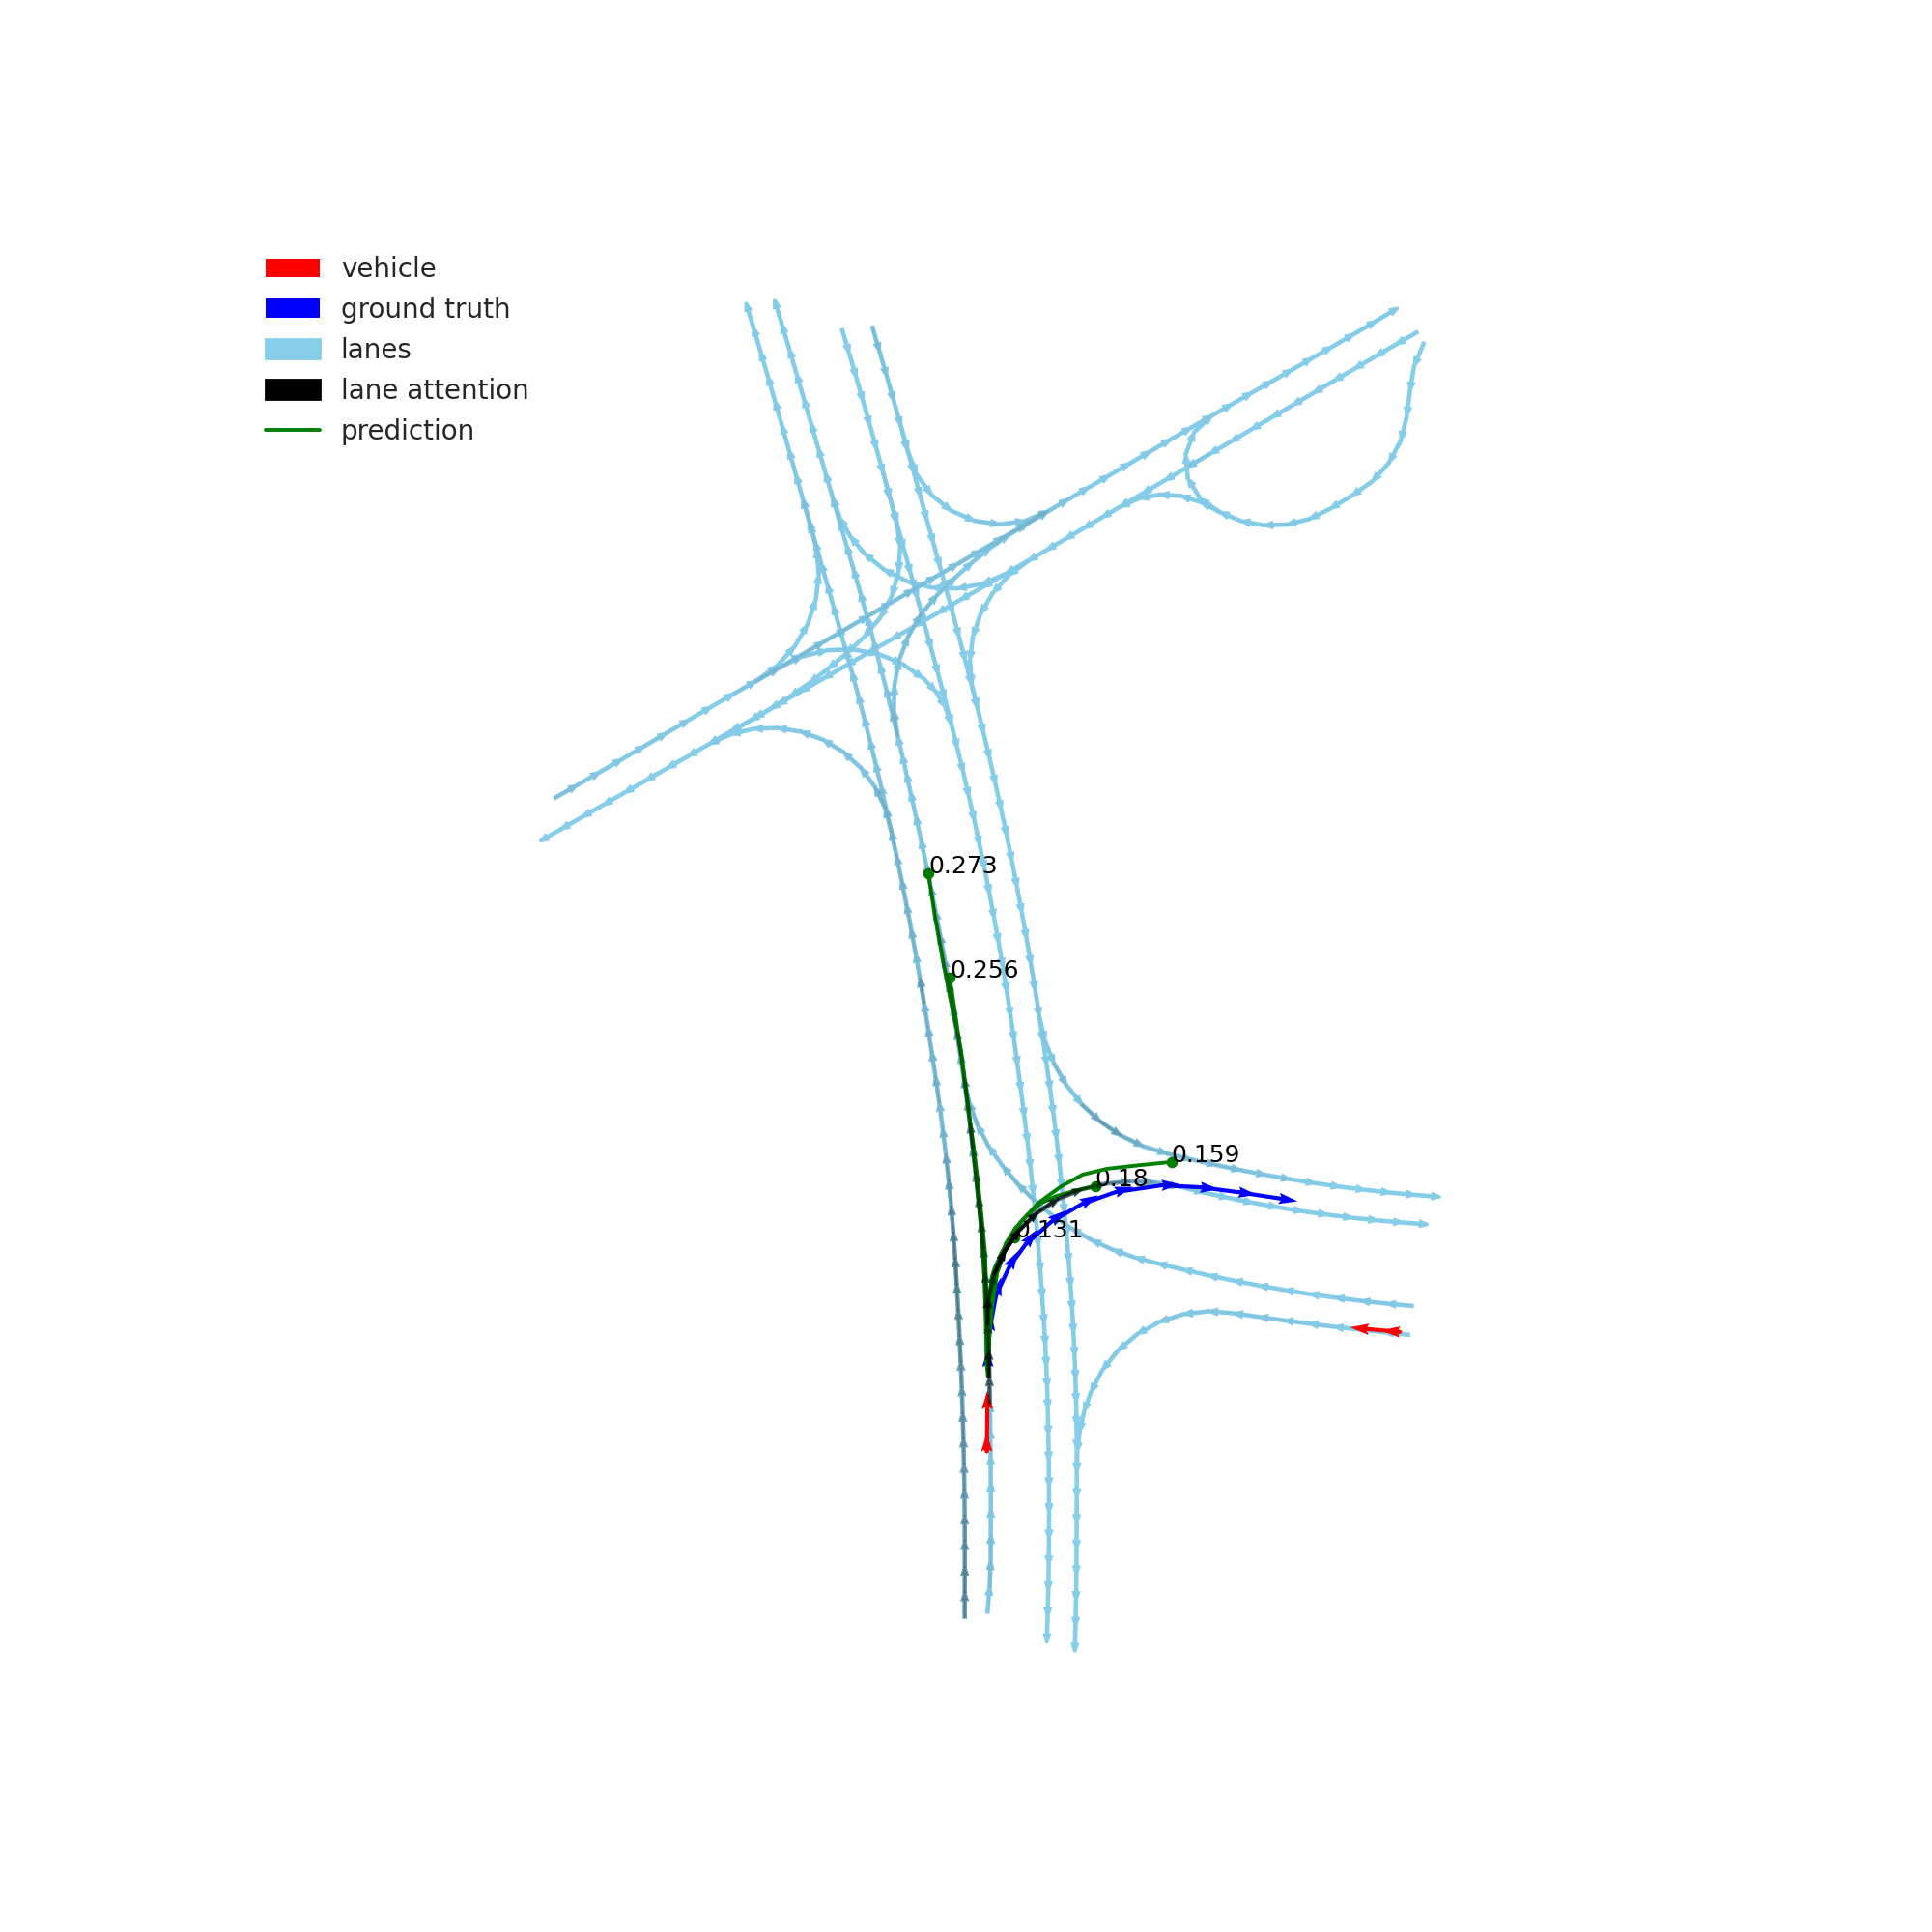
\includegraphics[height=4cm,trim={320 170 225 315},clip]{images_results/6f902cccc24d49a2b91d1d7f00047f83_6891260ad7c84844b5e74faf17303fff_minADE5_5.44_2-min.png}
    %     % \caption{Final Trajectories}
    % \end{subfigure}
    \begin{subfigure}[t]{0.4\linewidth}
        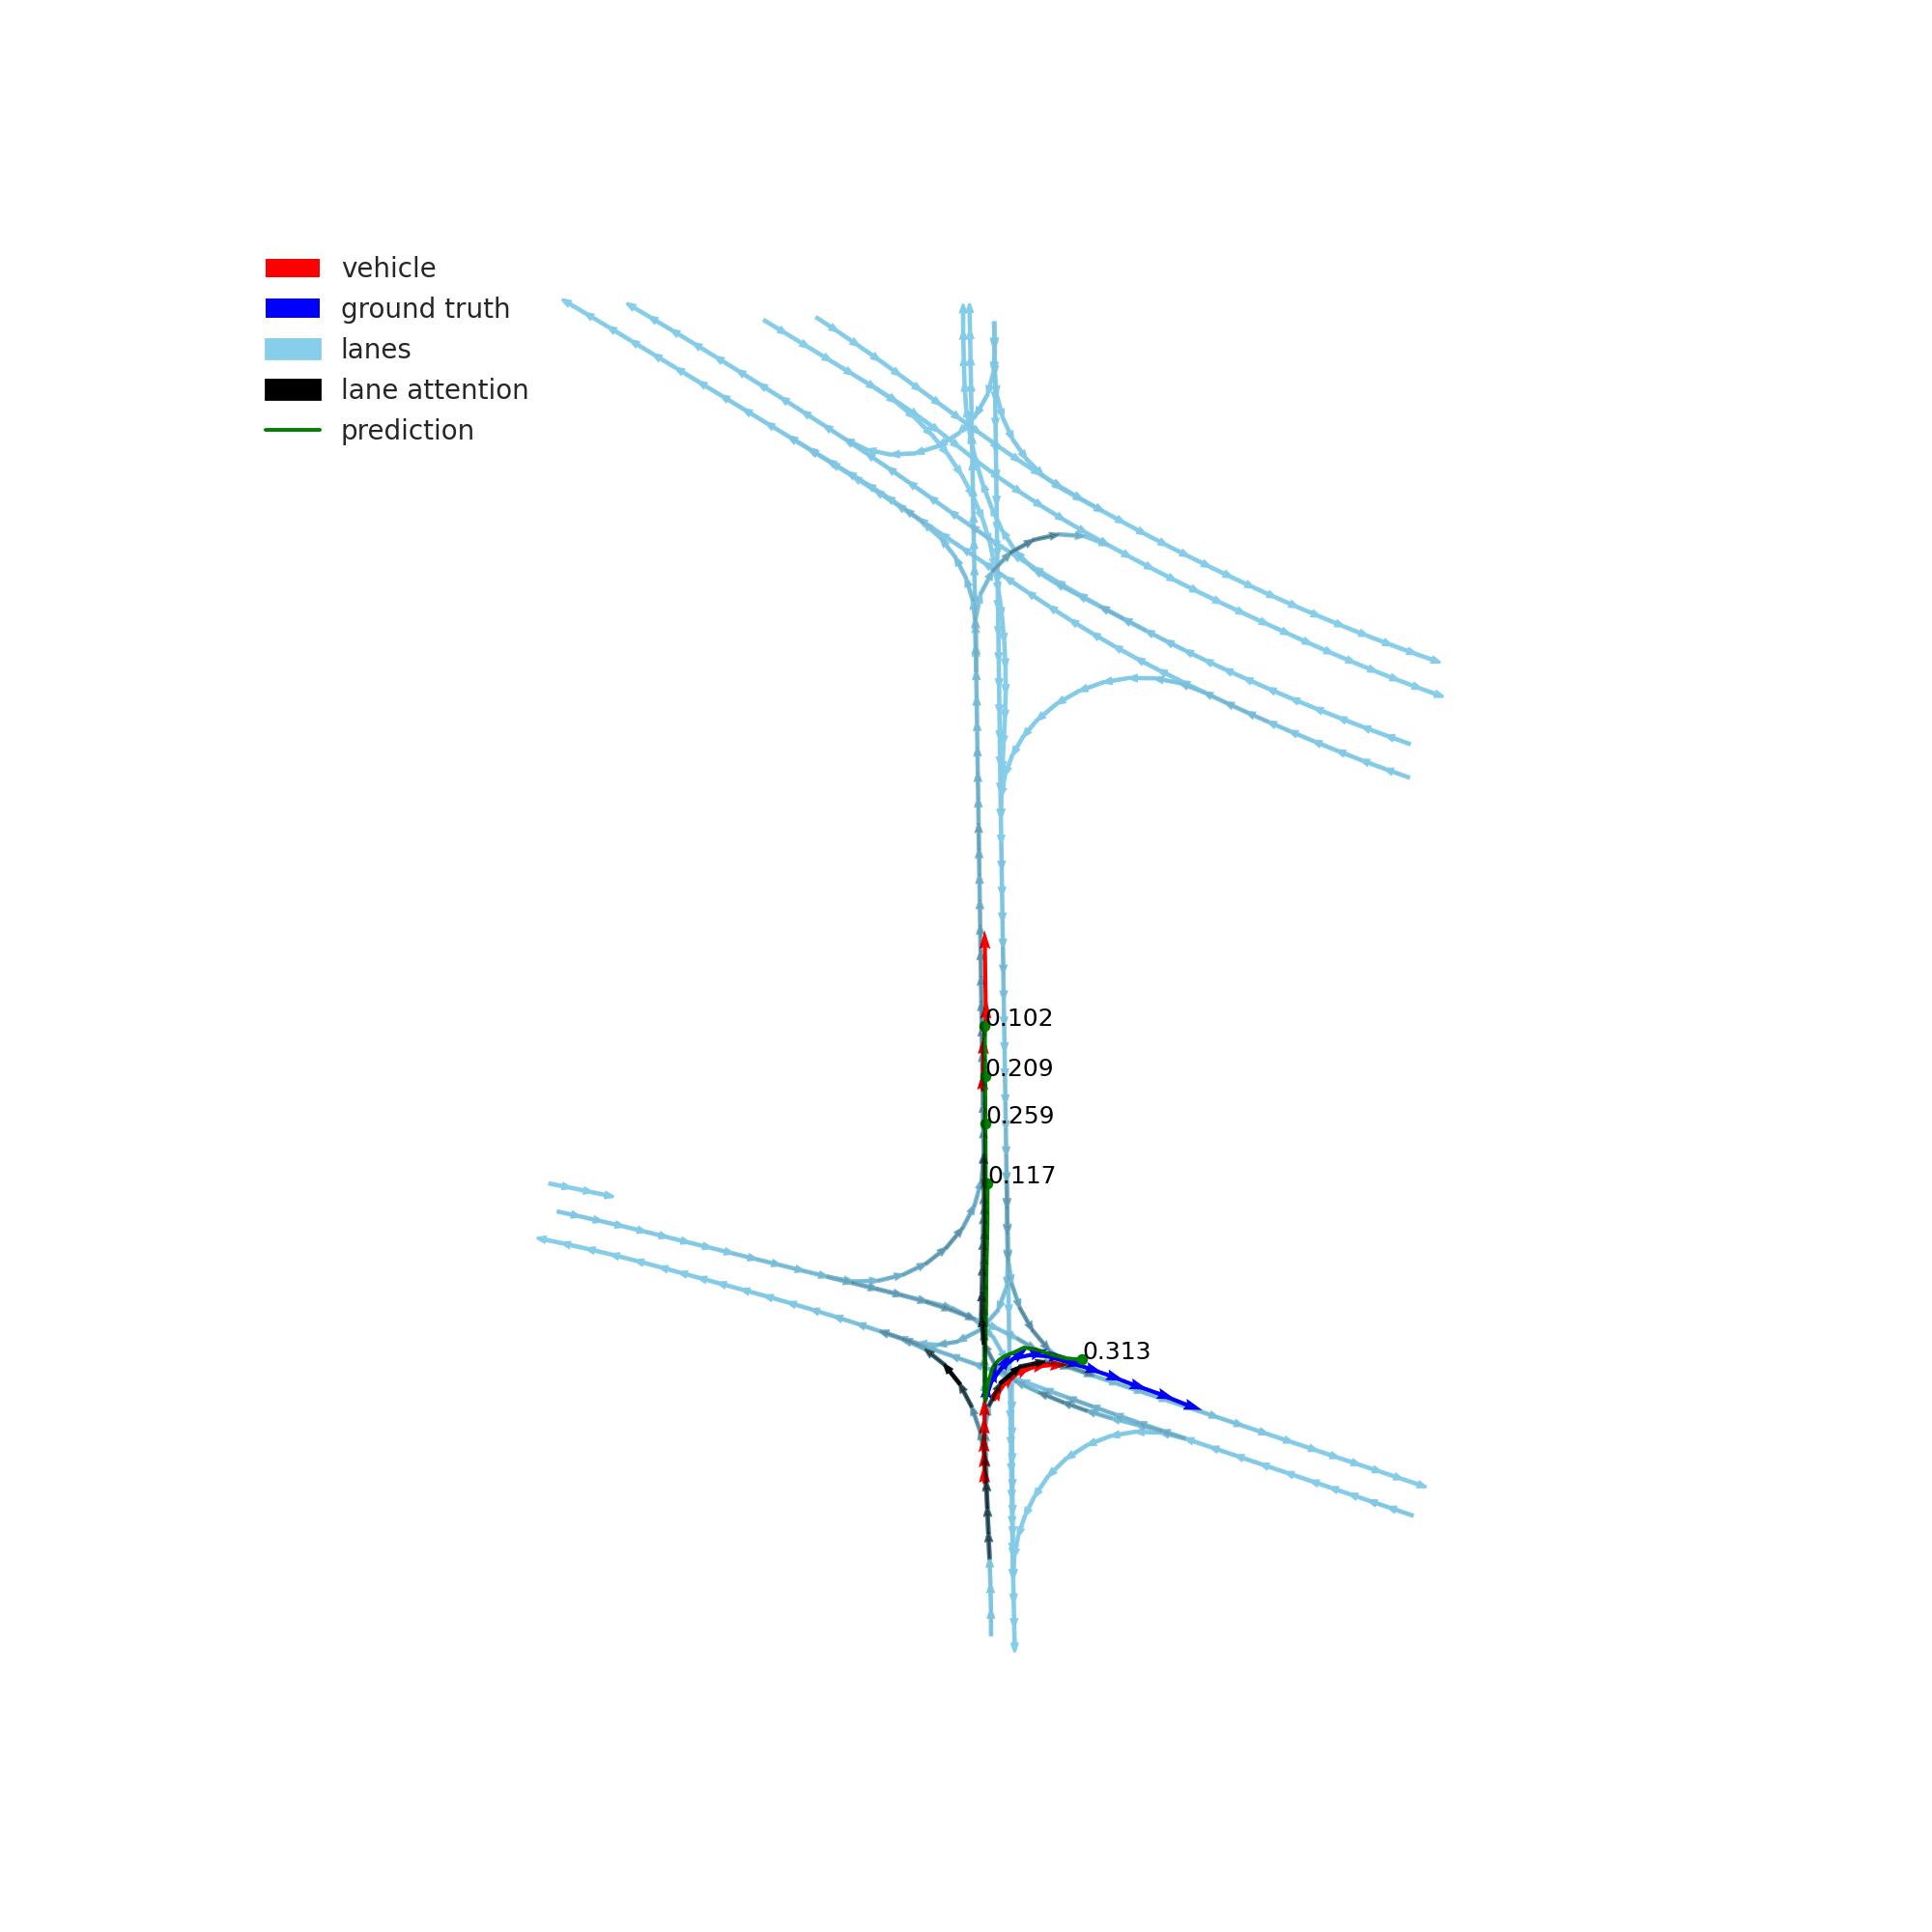
\includegraphics[height=4cm,trim={320 160 260 330},clip]{images_results/159dc0dc10134858aed2d6005da00b27_04147507f33e495f912cb64a60bb3f0d_minADE5_5.73_2-min.png}
        % \caption{Final Trajectories}
    \end{subfigure}
    \begin{tikzpicture}[remember picture,overlay]
      \node at (0, 3.3)      {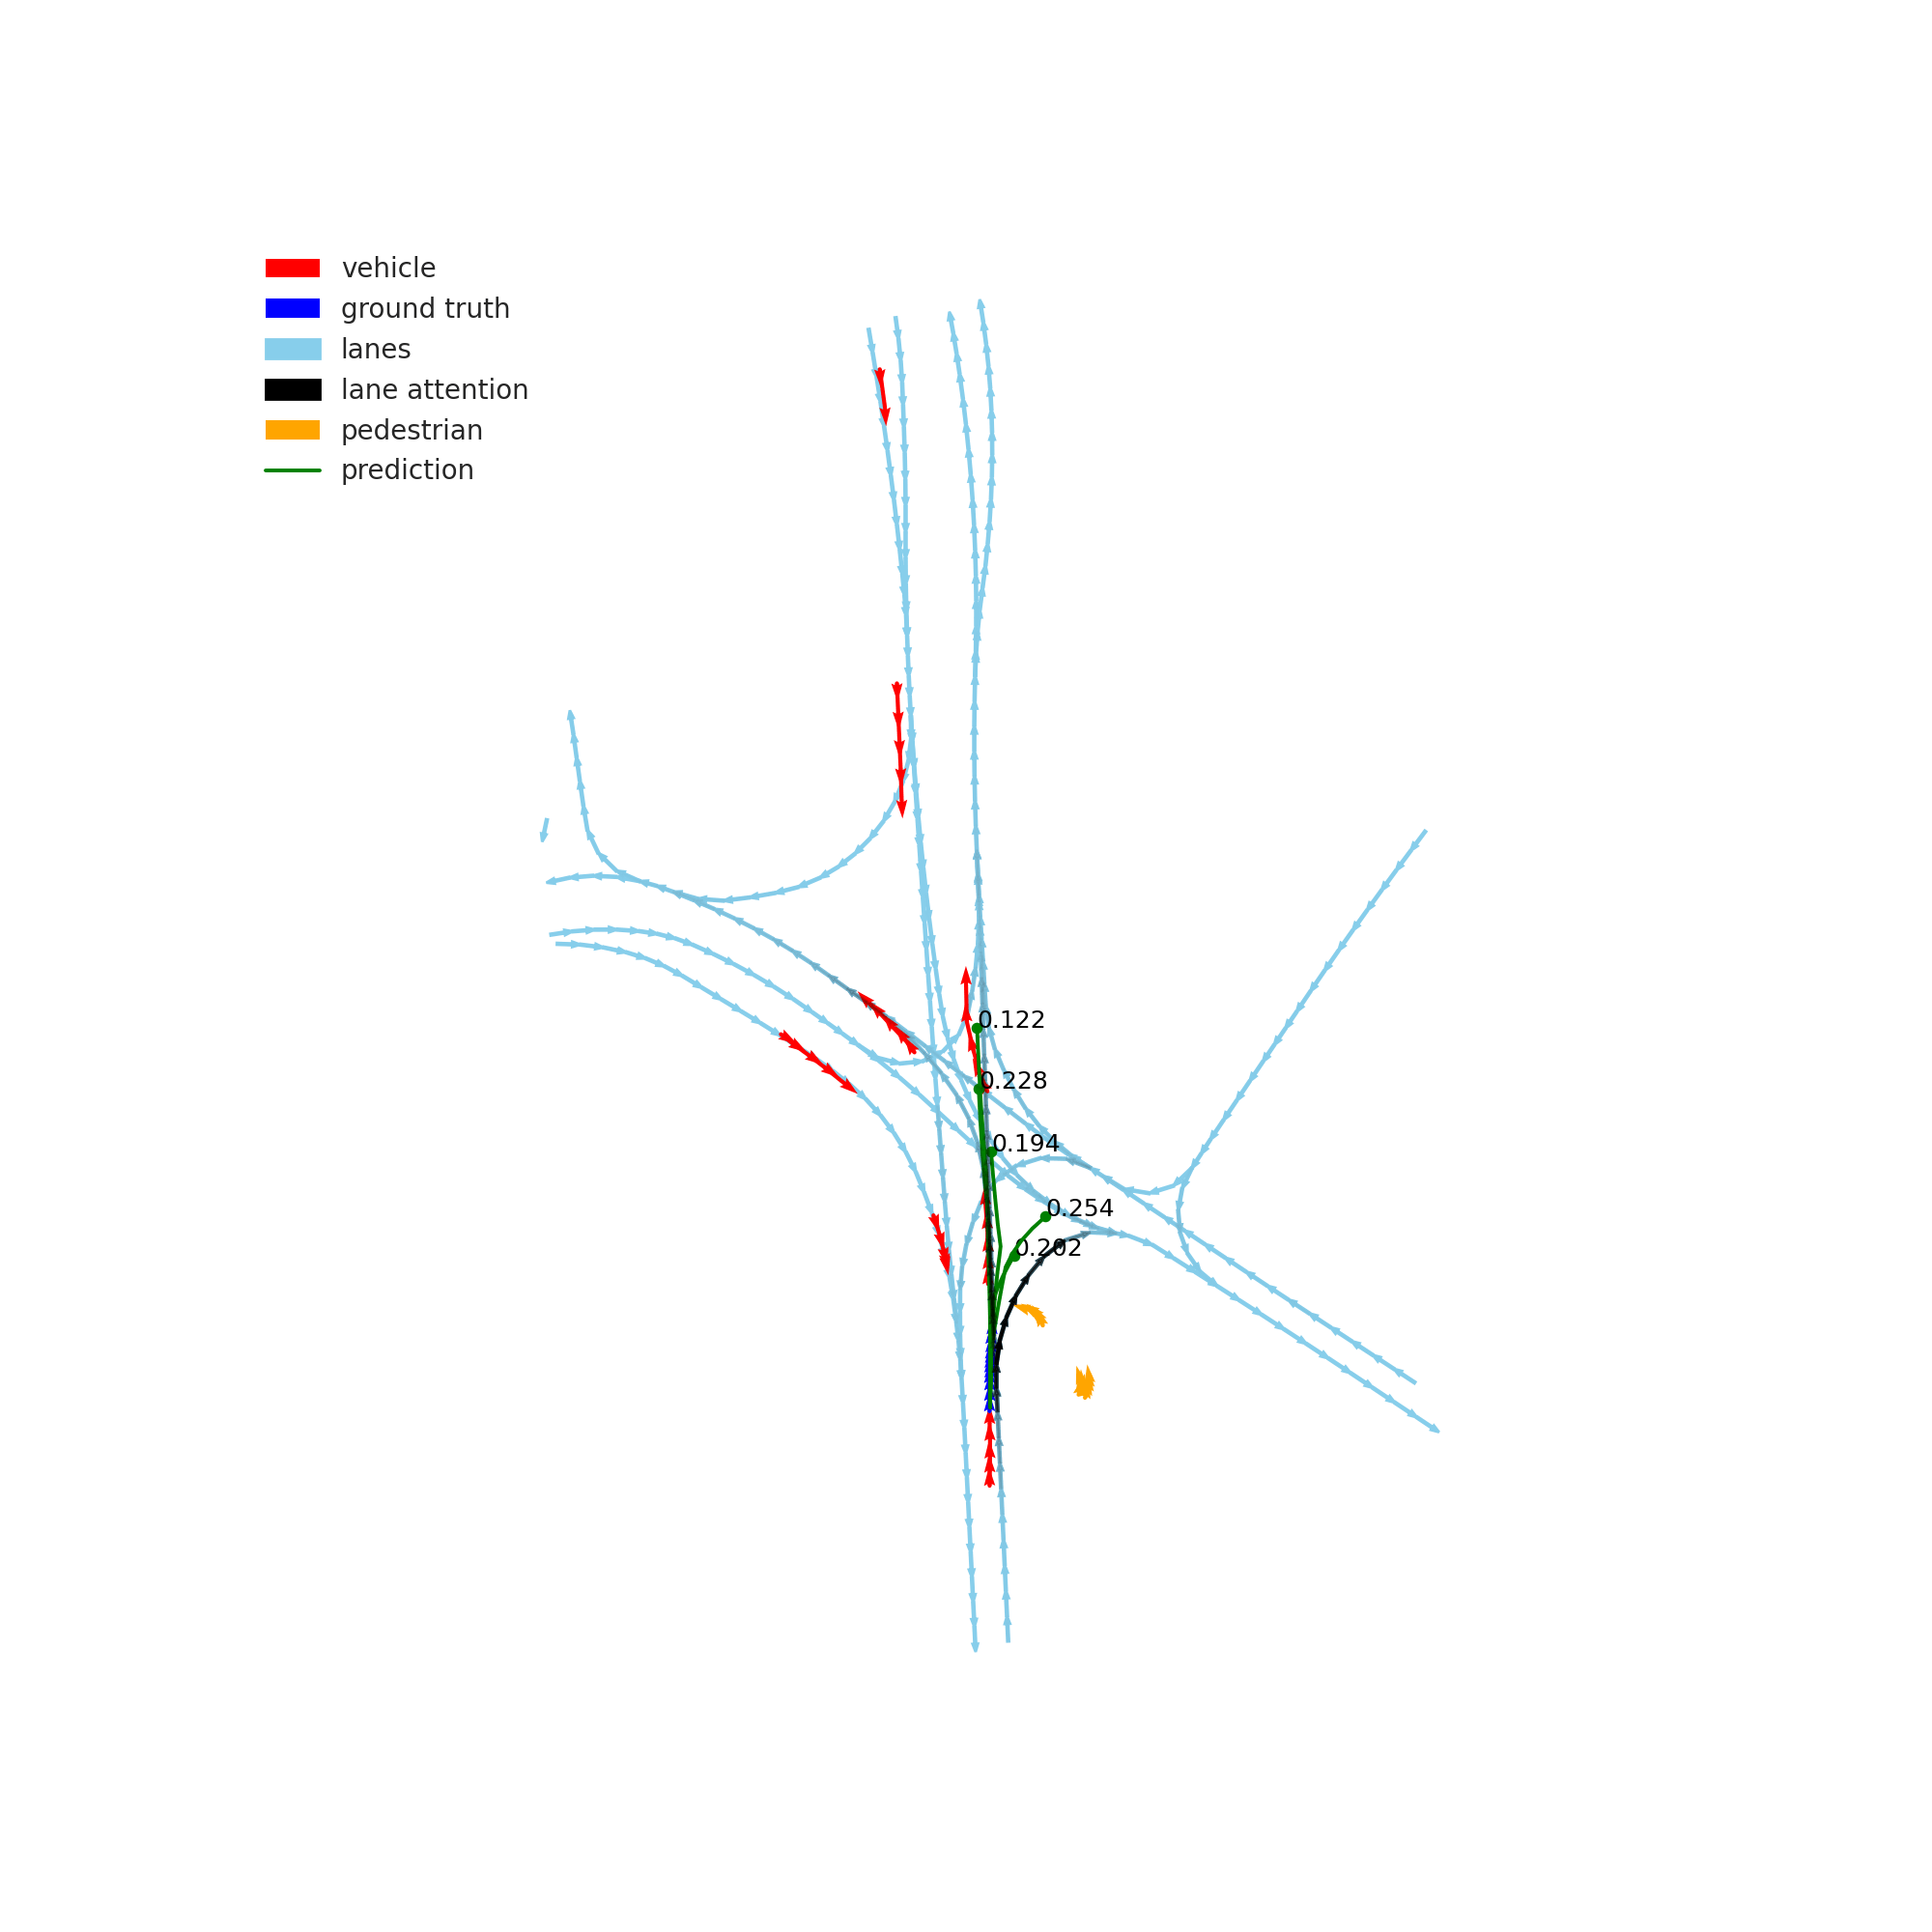
\includegraphics[width=0.23\linewidth,trim={110 500 450 85},clip]{images_results/2706cc4eb61844a1a5c7a5cb766ffc2e_37ab2d88d07846ef96d5227e9c5a15d7_minADE5_5.01_0-min.png}};
    \end{tikzpicture}
    \caption{An illustration of predicted trajectories (green) with mode probabilities for the target agent at the final output layer. These samples are selected out of the 100 worst predictions based on minADE\textsubscript{5}.}
    \label{fig:nuScenes_worst}    
\end{figure}

We also test the generalization capability of LMFormer on the Deep Scenario dataset \cite{lu2023deepscenario}. To this end, we train the network on 55,000 training samples, generated from four different intersections' recordings ('Unparalleled Frankfurt', 'Trendy Renningen', Fortunate Karlsruhe', 'Stunning Stuttgart') in the dataset. We conducted the qualitative testing for this model checkpoint on the samples of unobserved intersections during training (refer Figure \ref{fig:cross_data_qual}). We observe that in certain cases, LMFormer fails to predict all plausible trajectories. We hypothesize that this limitation is due to an unbalanced data distribution, where some maneuvers occur less frequently in the training data. This suggests that additional mechanisms, such as explicit trajectory diversity constraints or targeted data augmentation, may be required to improve the robustness of multimodal prediction, but we leave these improvements for future work.

\begin{figure}
    \centering
    \begin{subfigure}[t]{0.3\linewidth}
        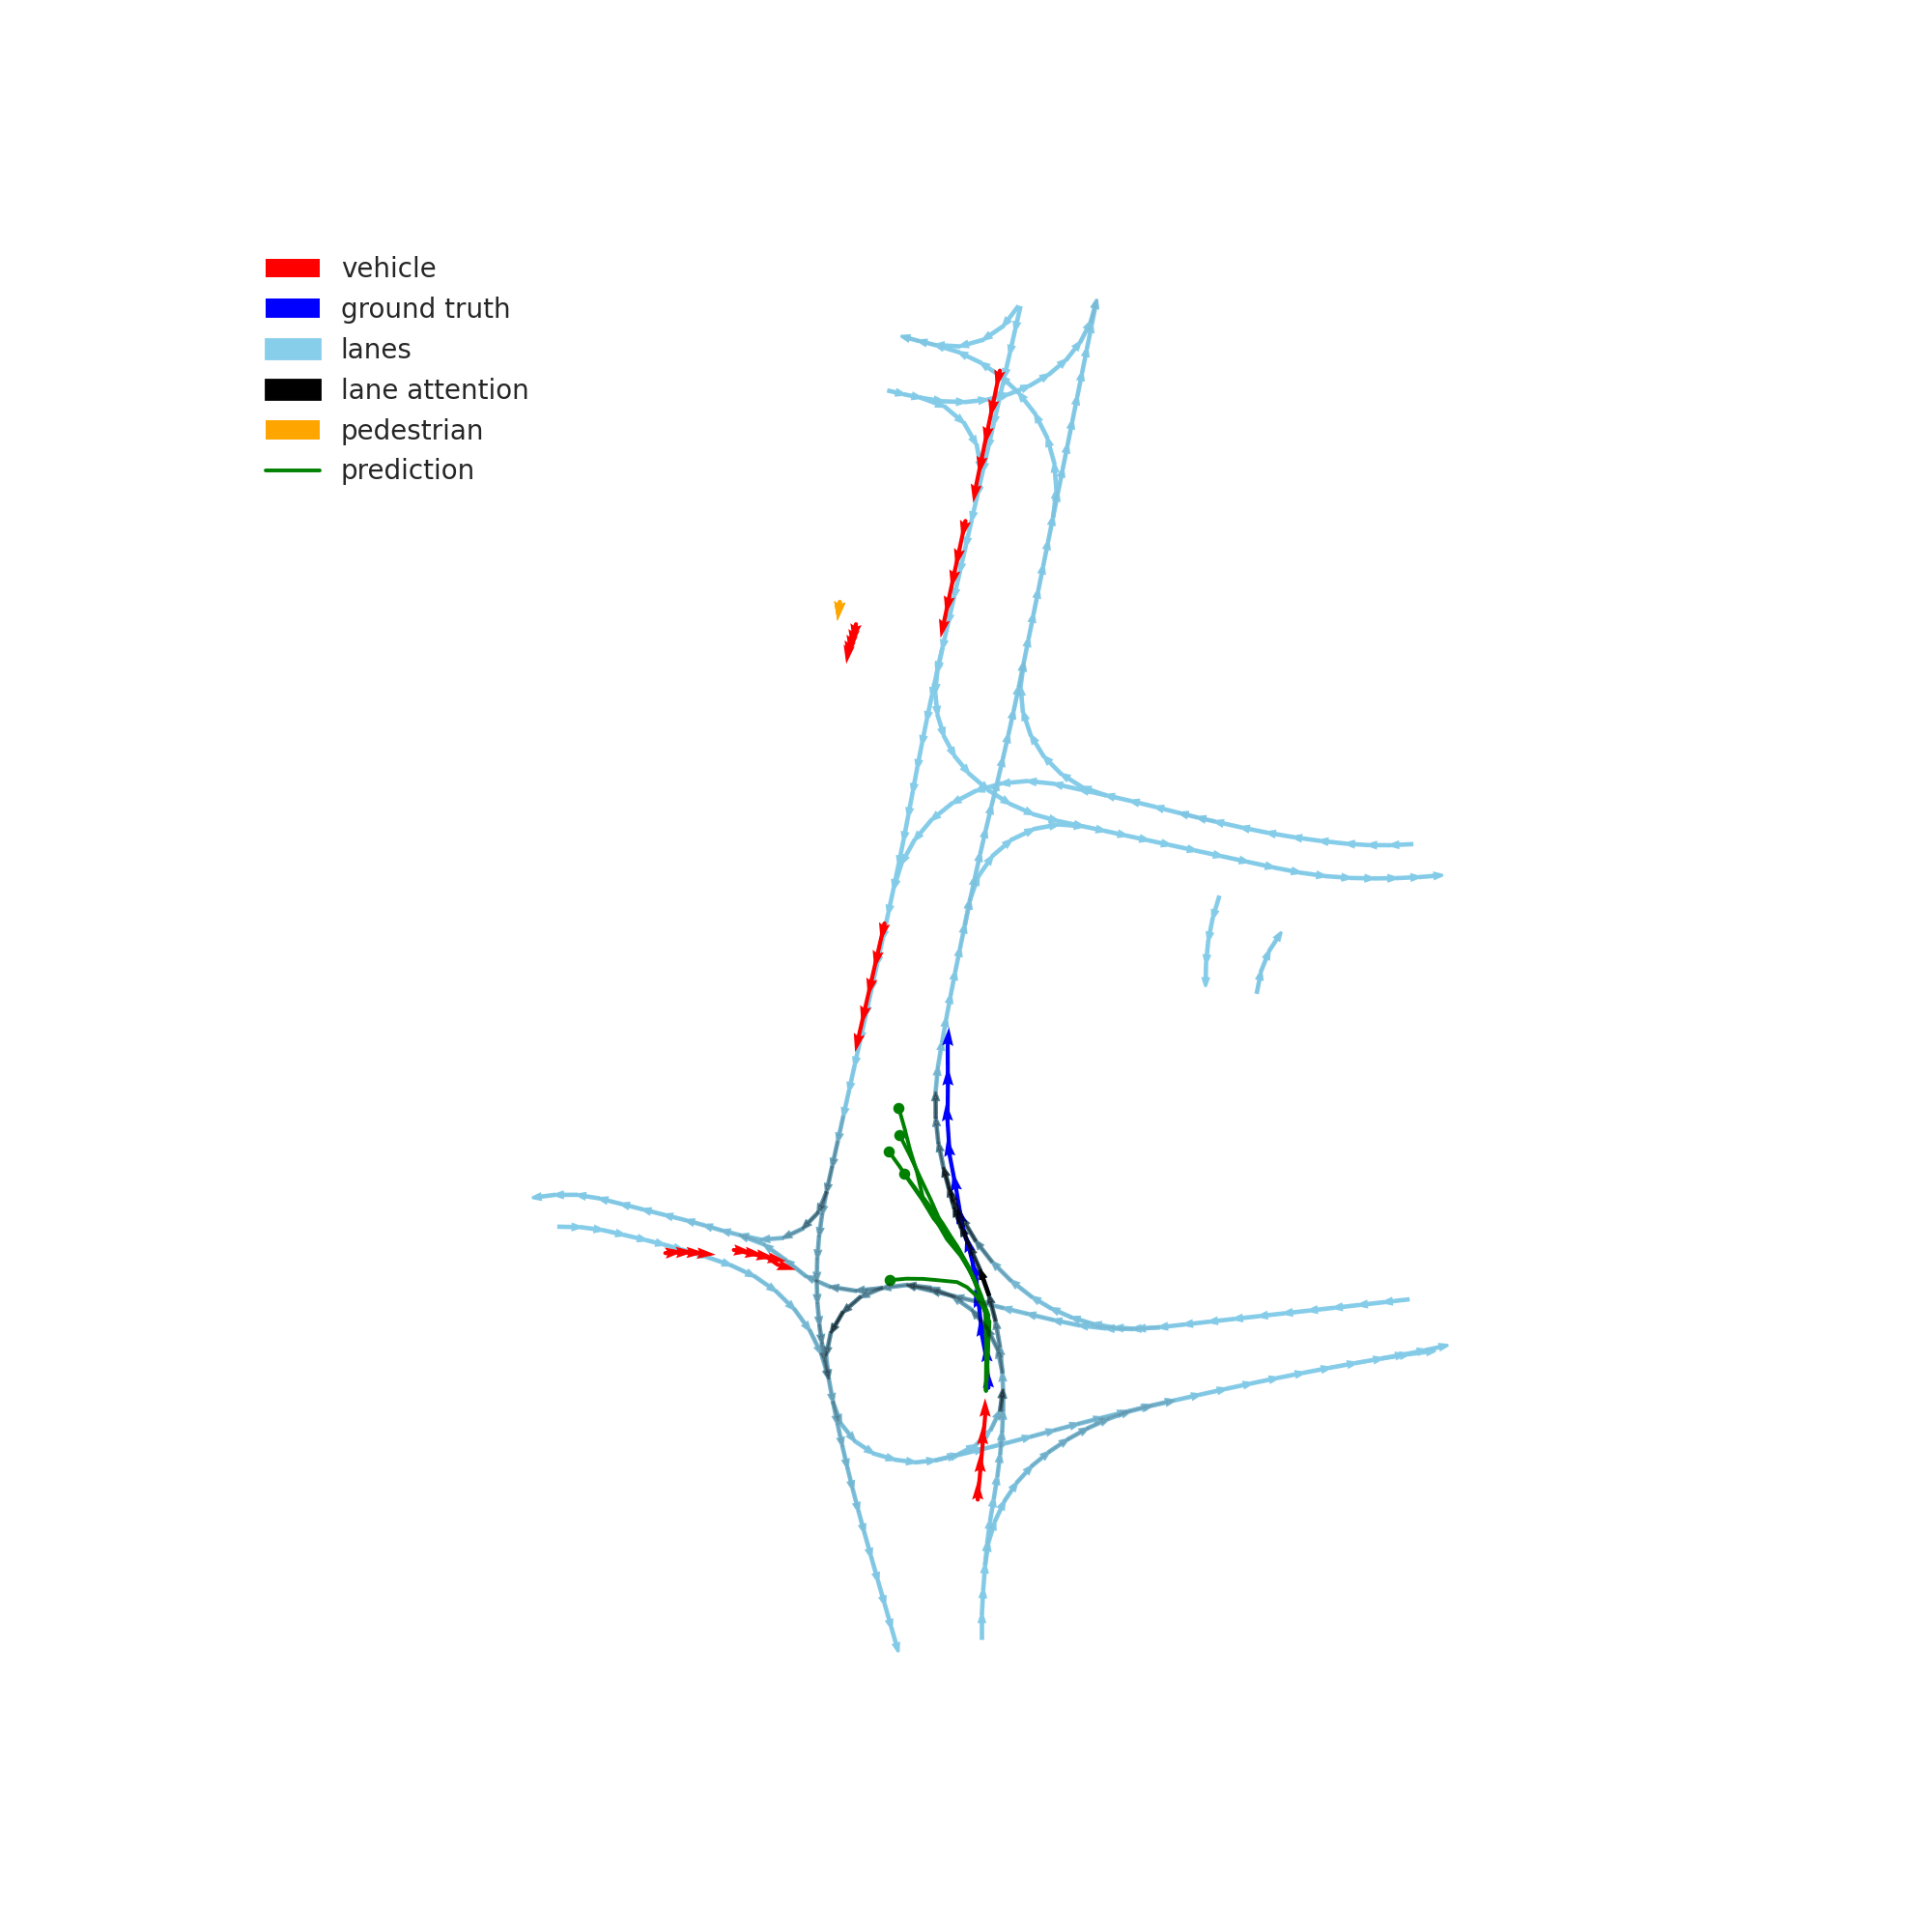
\includegraphics[height=3cm,trim={280 160 300 370},clip]{images_results/56d0094604014dee90a4dfb6f861f4e6_80e84ccf181a428e939af2fbde7d4211_0-min.png}
    \end{subfigure}
    \begin{subfigure}[t]{0.3\linewidth}
        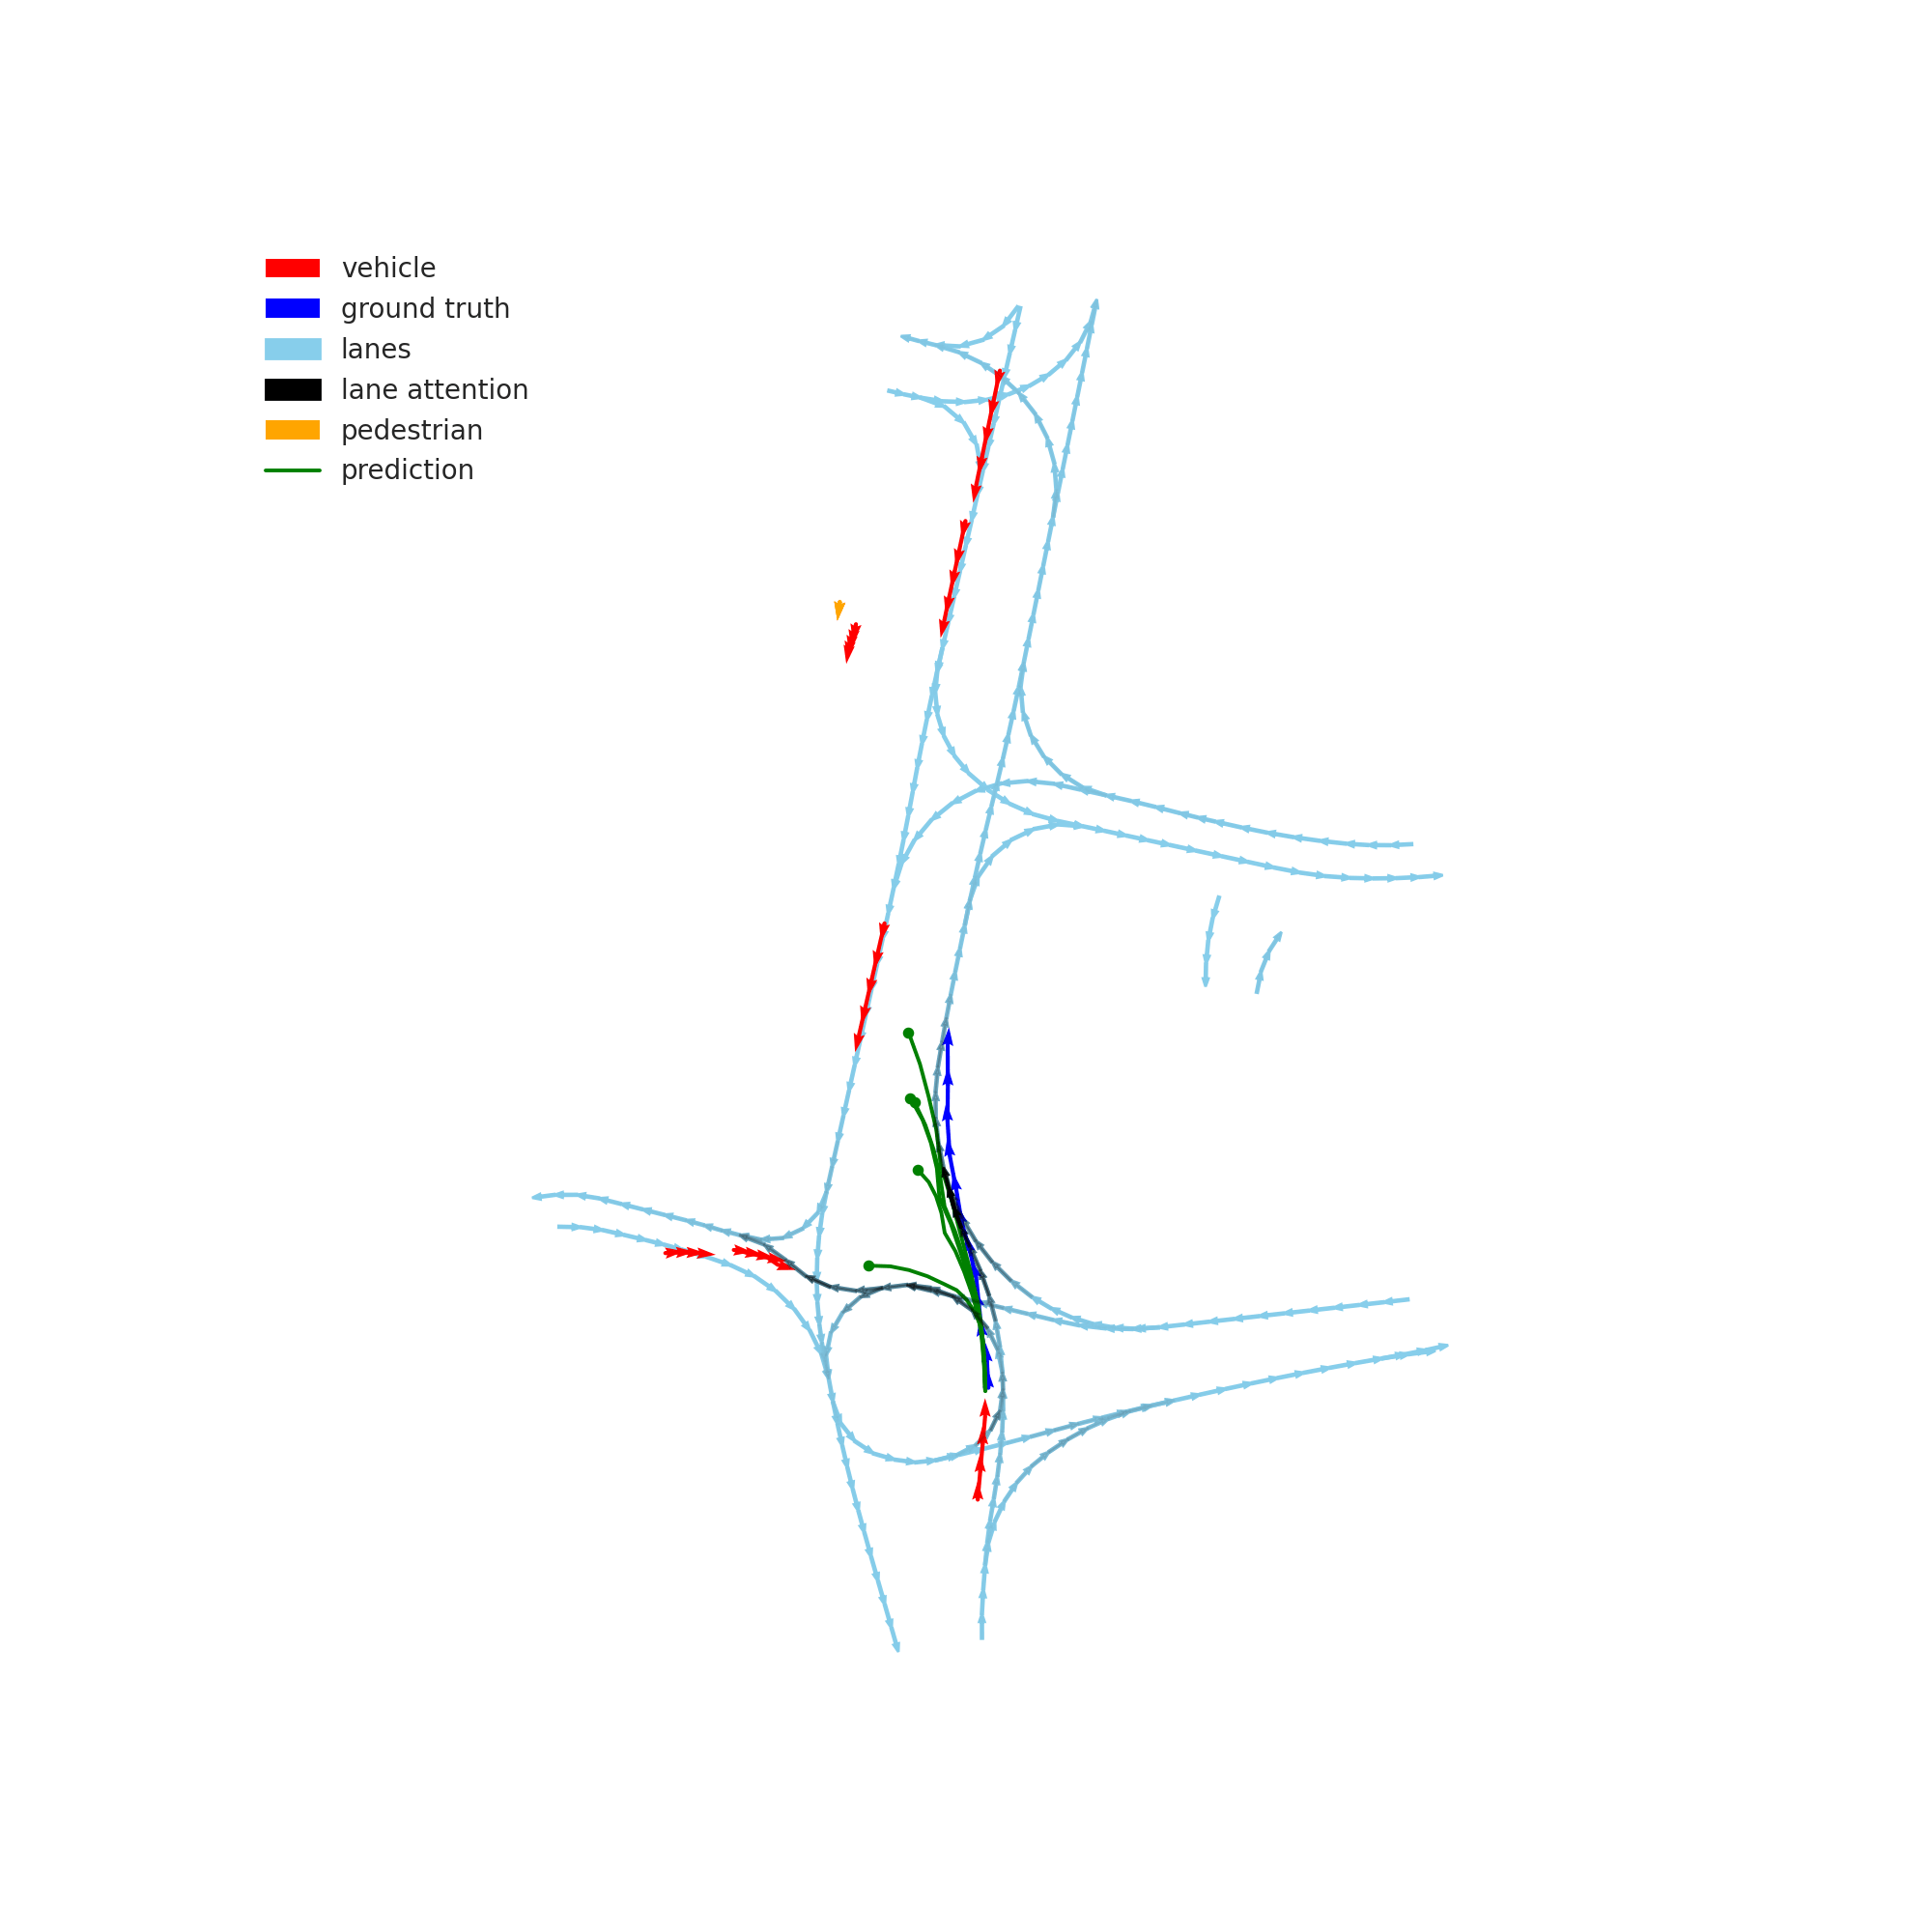
\includegraphics[height=3cm,trim={280 160 300 370},clip]{images_results/56d0094604014dee90a4dfb6f861f4e6_80e84ccf181a428e939af2fbde7d4211_1-min.png}
    \end{subfigure}
    \begin{subfigure}[t]{0.3\linewidth}
        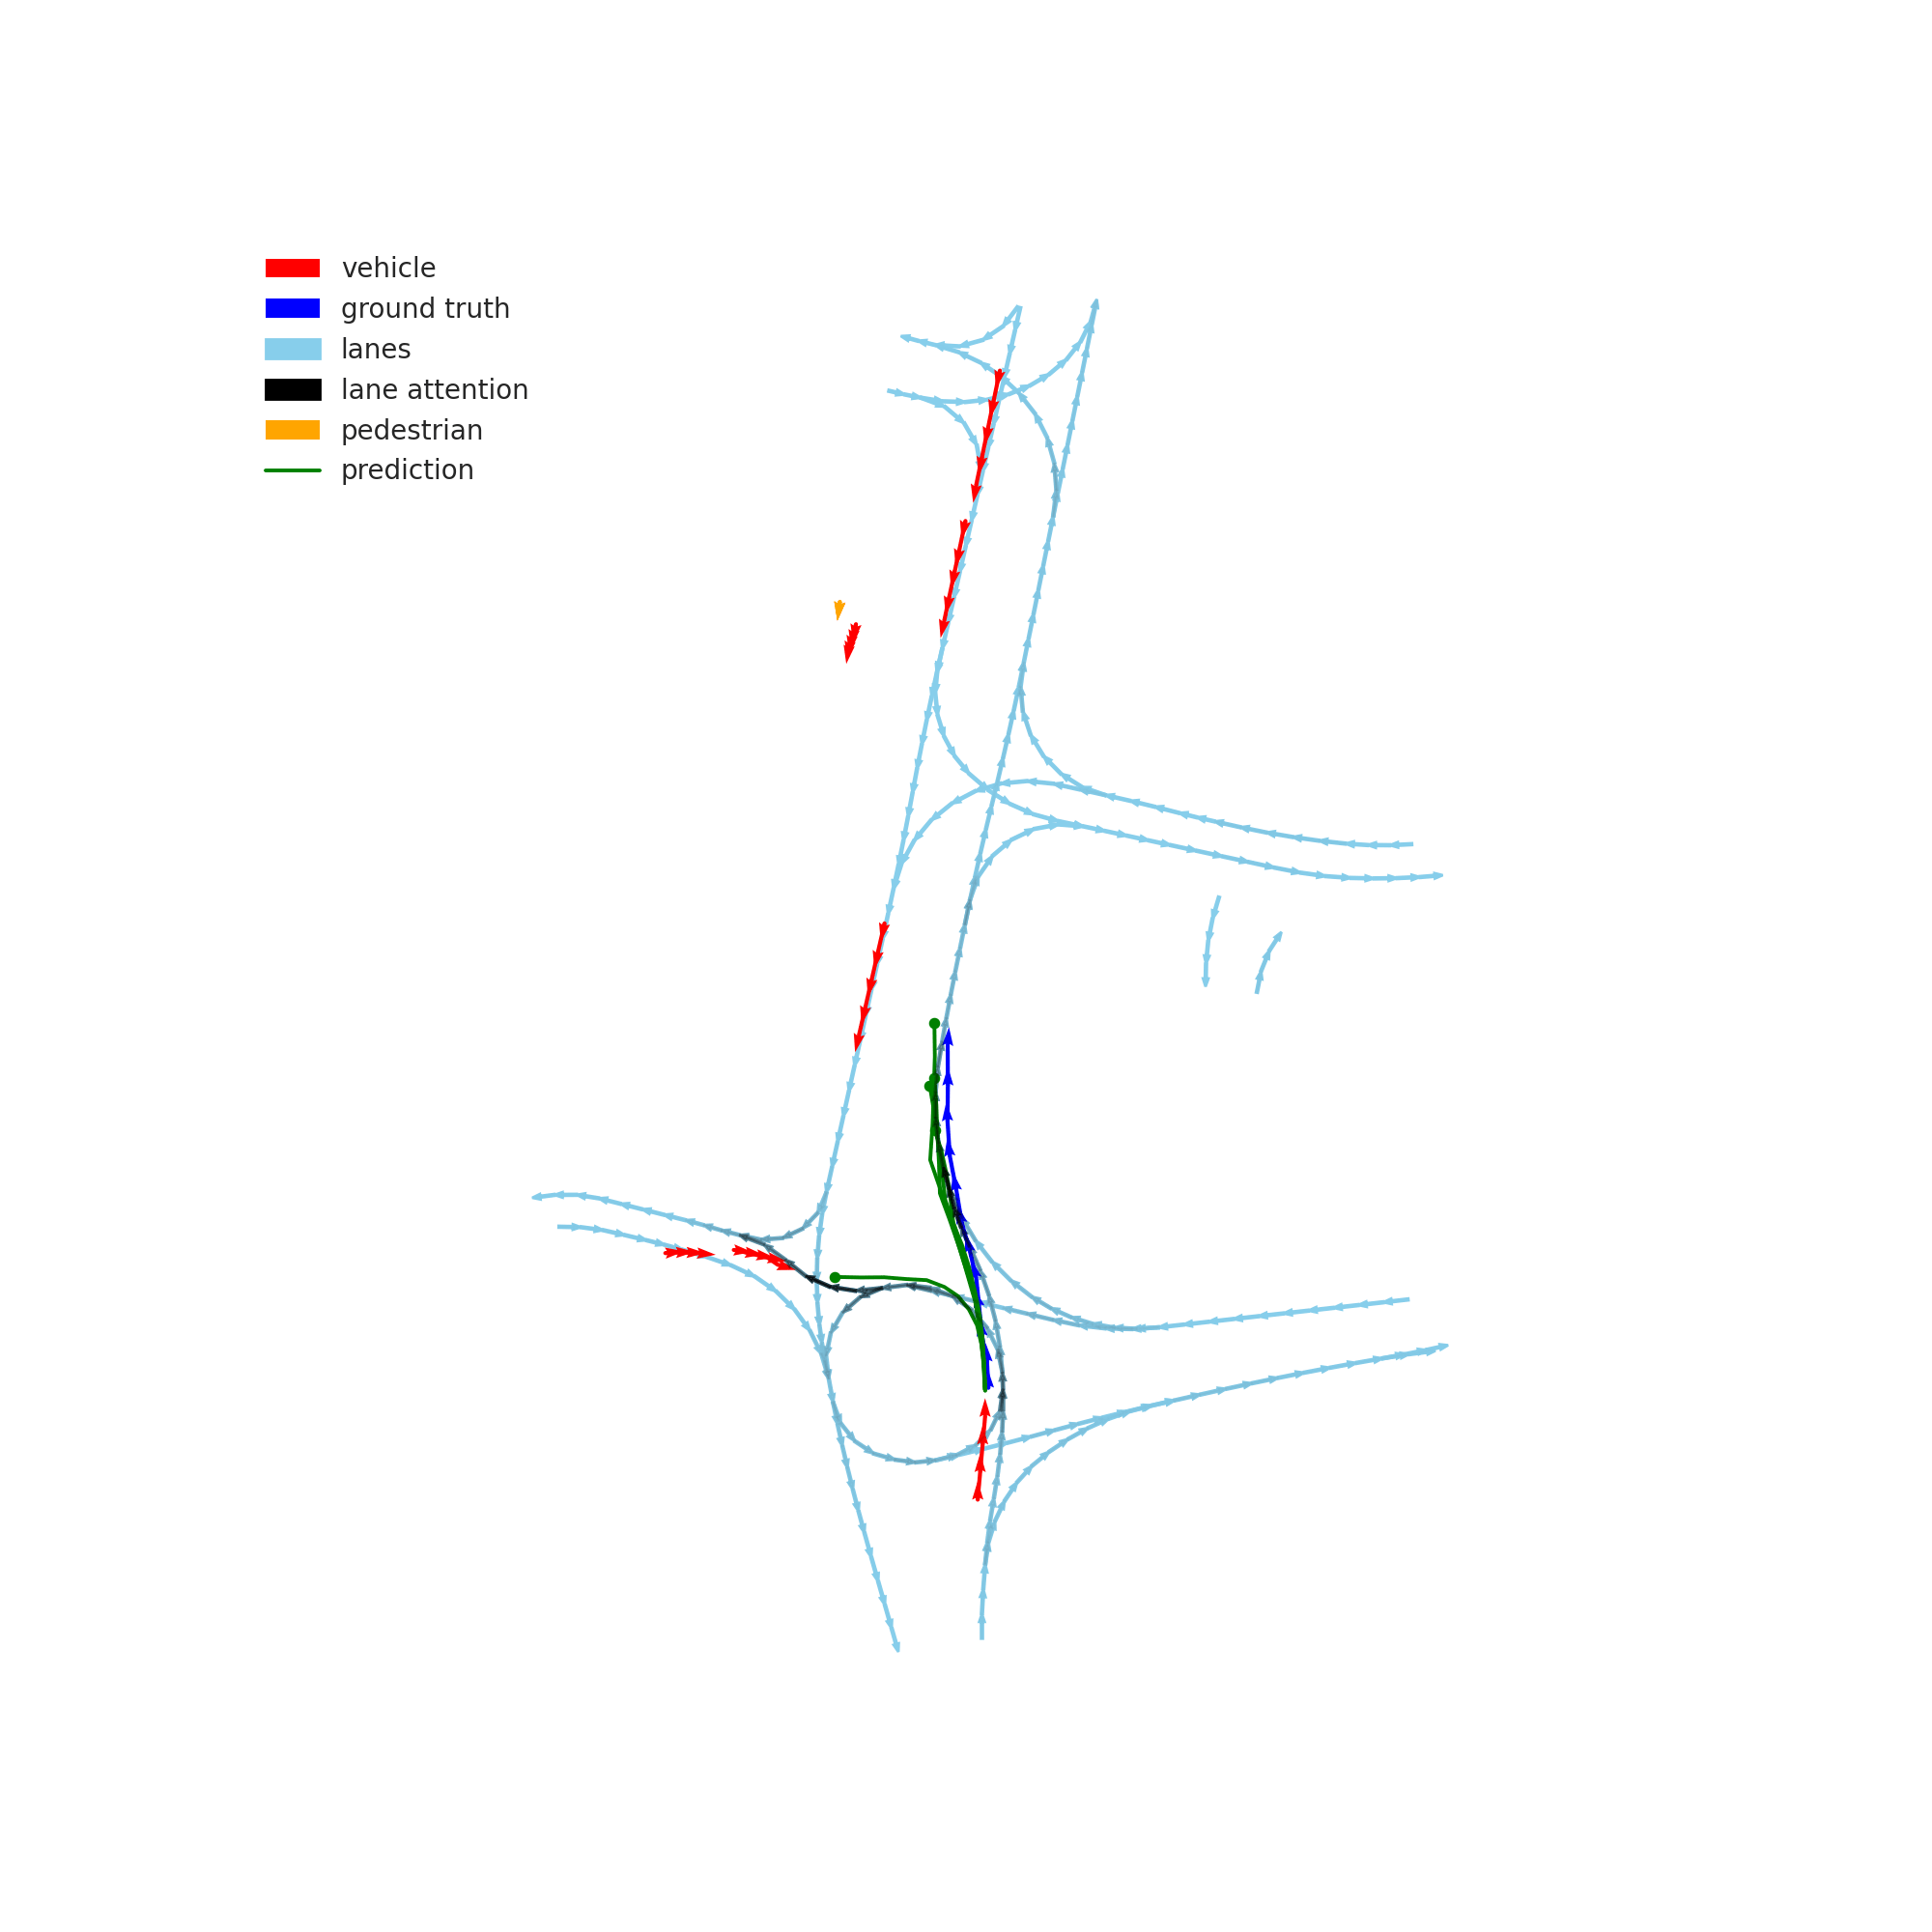
\includegraphics[height=3cm,trim={280 160 300 370},clip]{images_results/56d0094604014dee90a4dfb6f861f4e6_80e84ccf181a428e939af2fbde7d4211_2-min.png}
    \end{subfigure}
    \begin{subfigure}[t]{0.3\linewidth}
        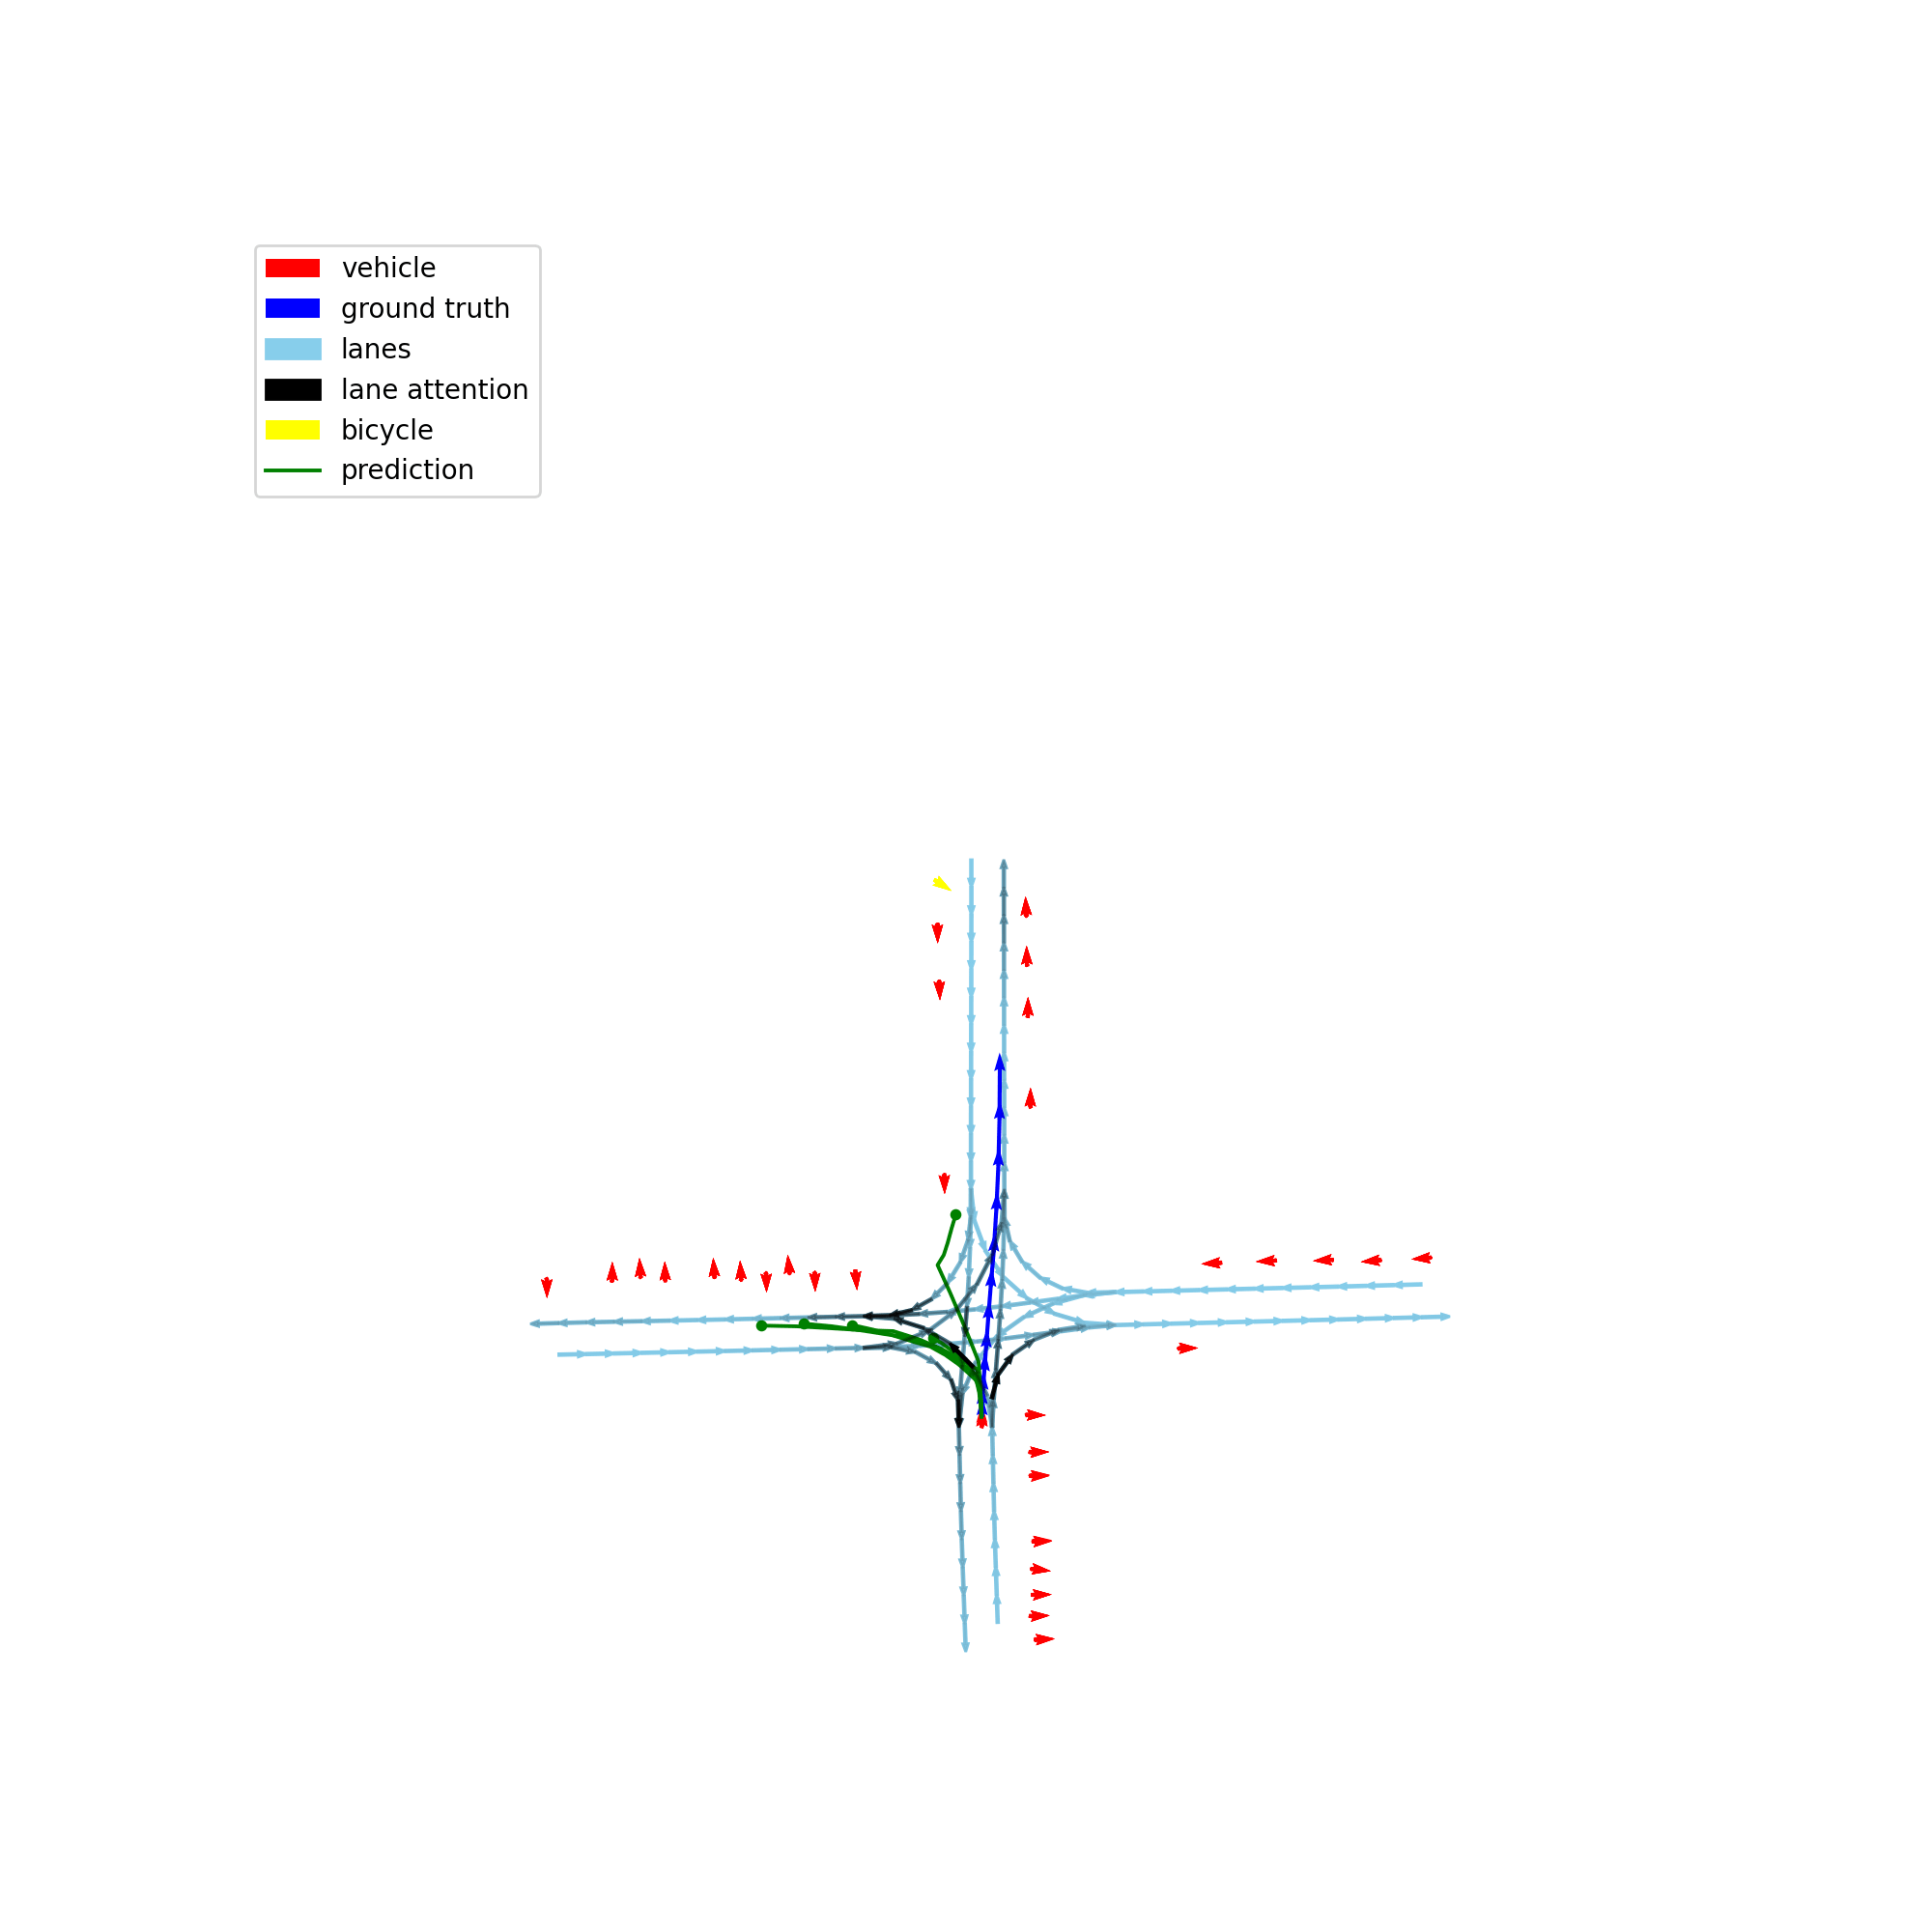
\includegraphics[height=3cm,trim={280 170 300 380},clip]{images_results/1337_minADE5_9.3_0-min.png}
        \caption{Initial}
    \end{subfigure}
    \begin{subfigure}[t]{0.3\linewidth}
        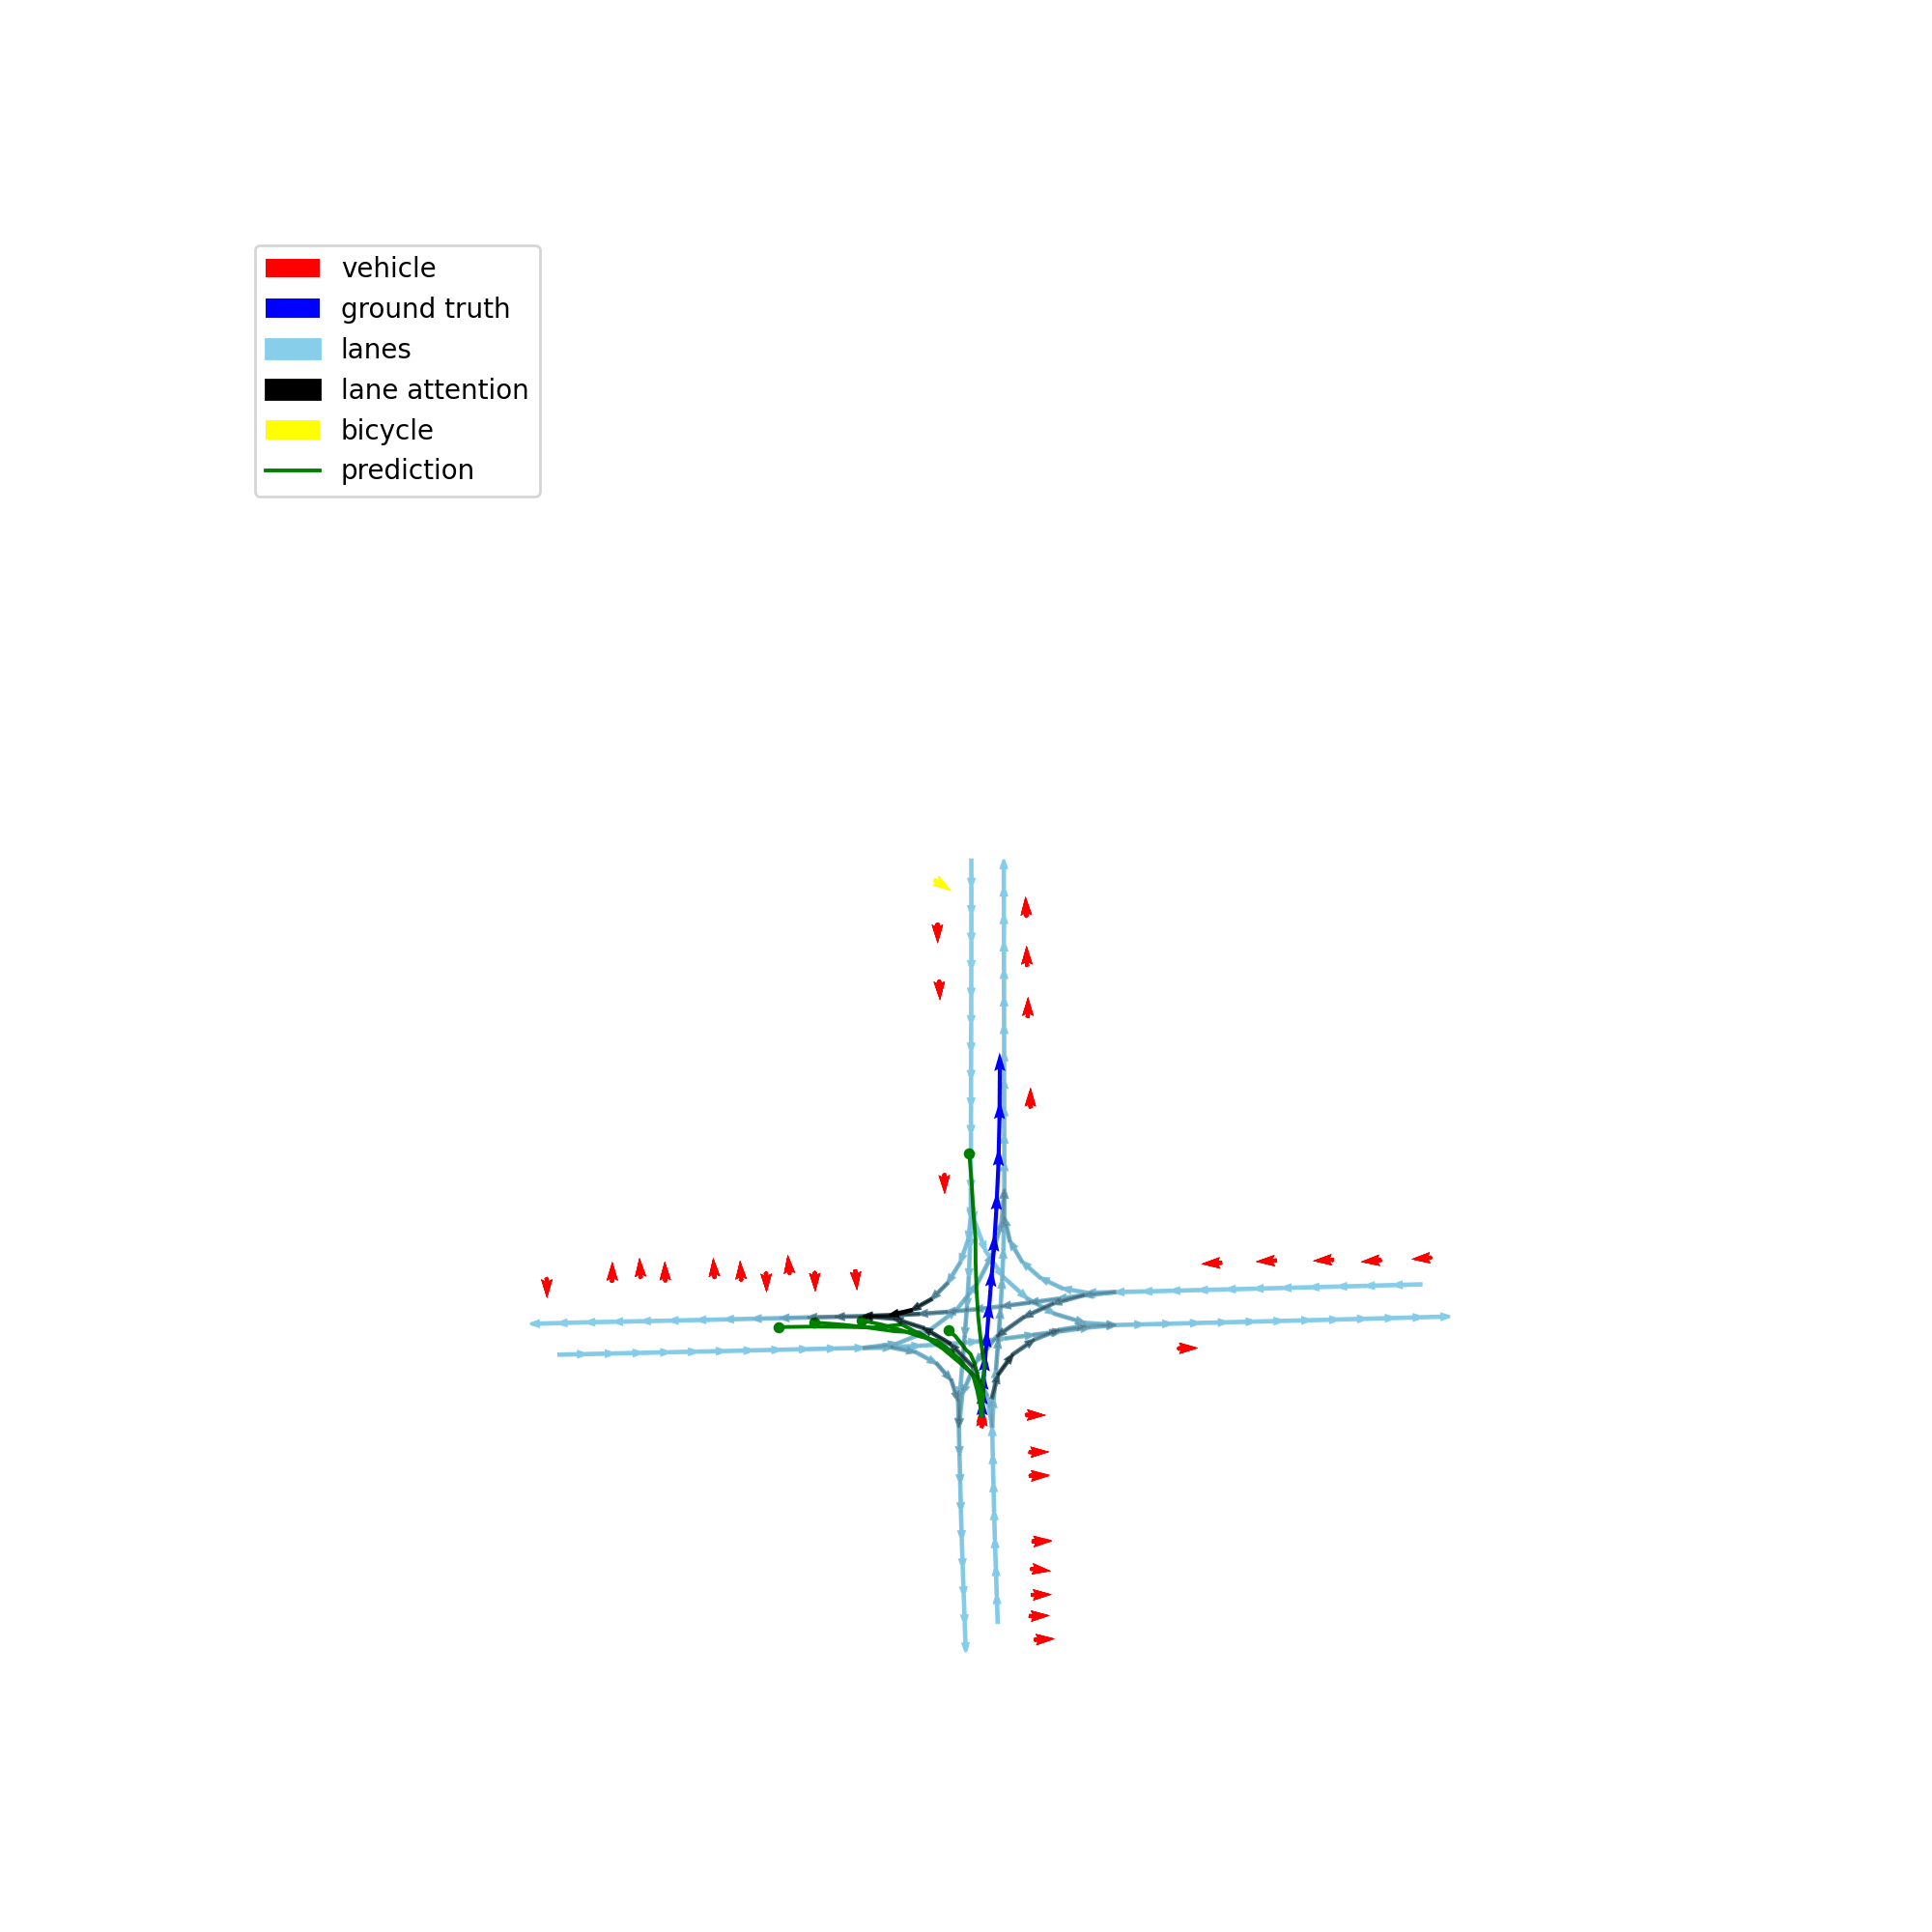
\includegraphics[height=3cm,trim={280 170 300 380},clip]{images_results/1337_minADE5_9.3_1-min.png}
        \caption{Refinement}
    \end{subfigure}
    \begin{subfigure}[t]{0.3\linewidth}
        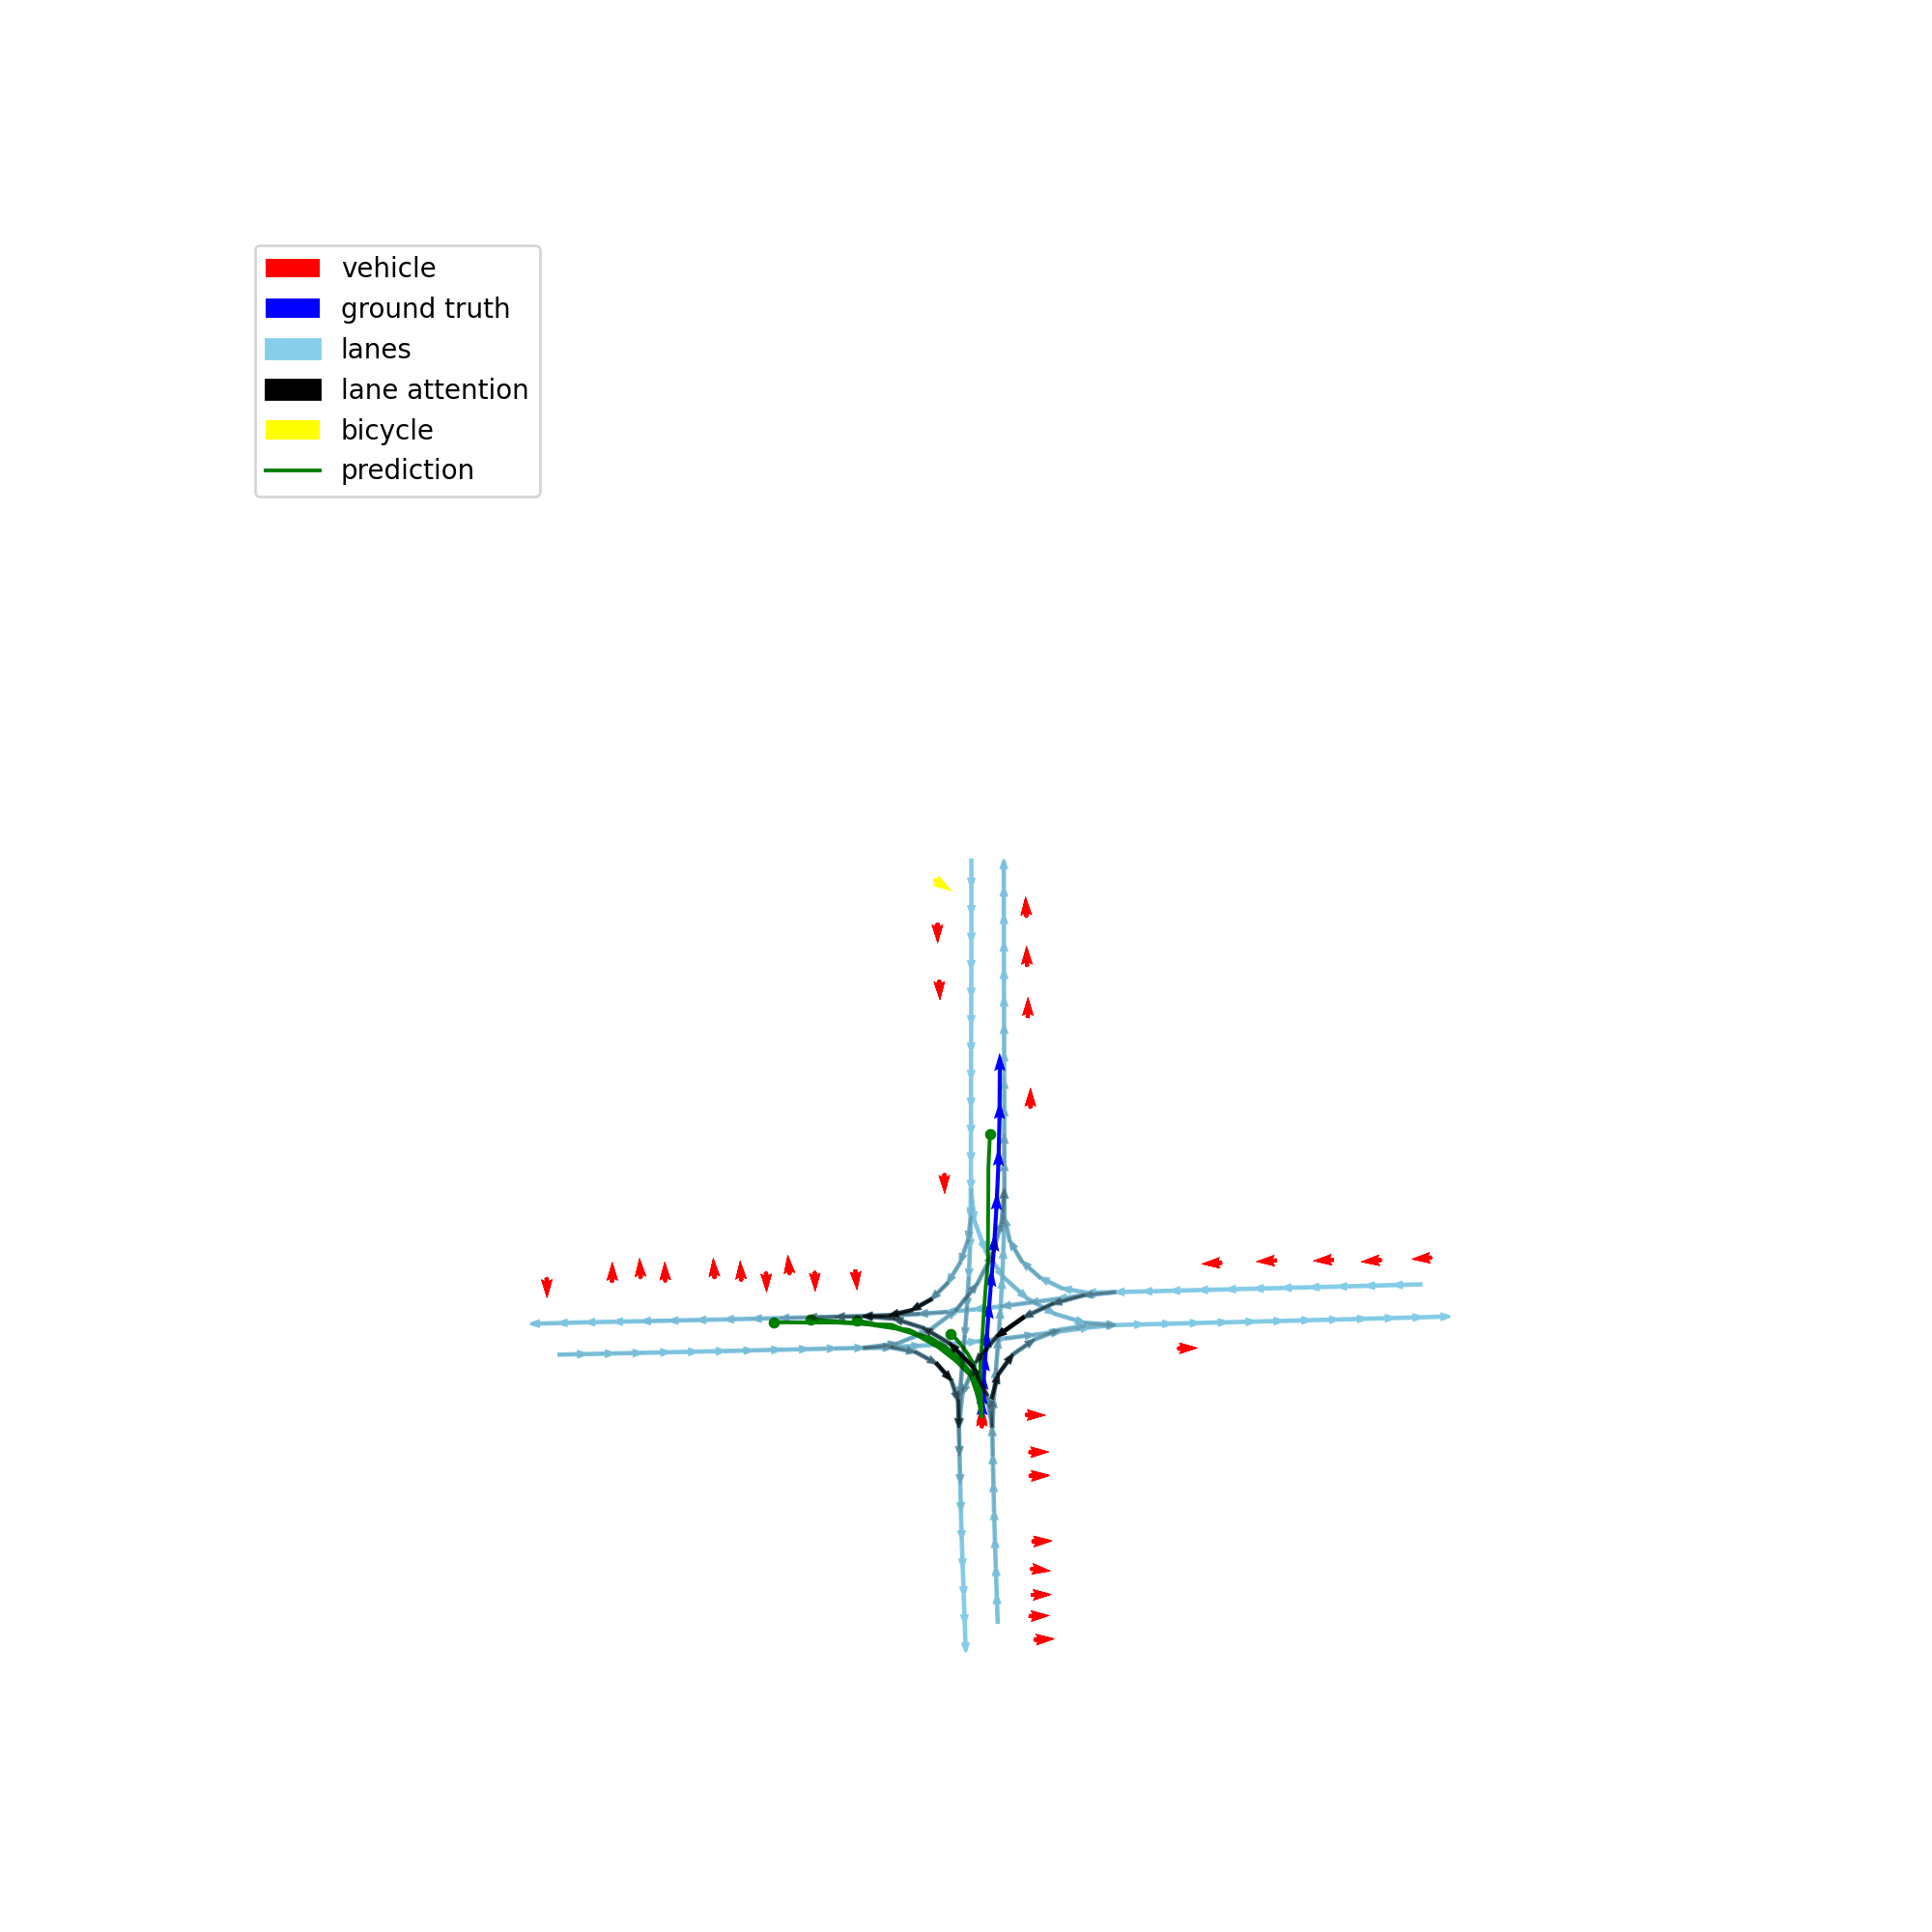
\includegraphics[height=3cm,trim={280 170 300 380},clip]{images_results/1337_minADE5_9.3_2-min.png}
        \caption{Final}
    \end{subfigure}
    % \begin{tikzpicture}[remember picture,overlay]
    %  \node at (0,3)      {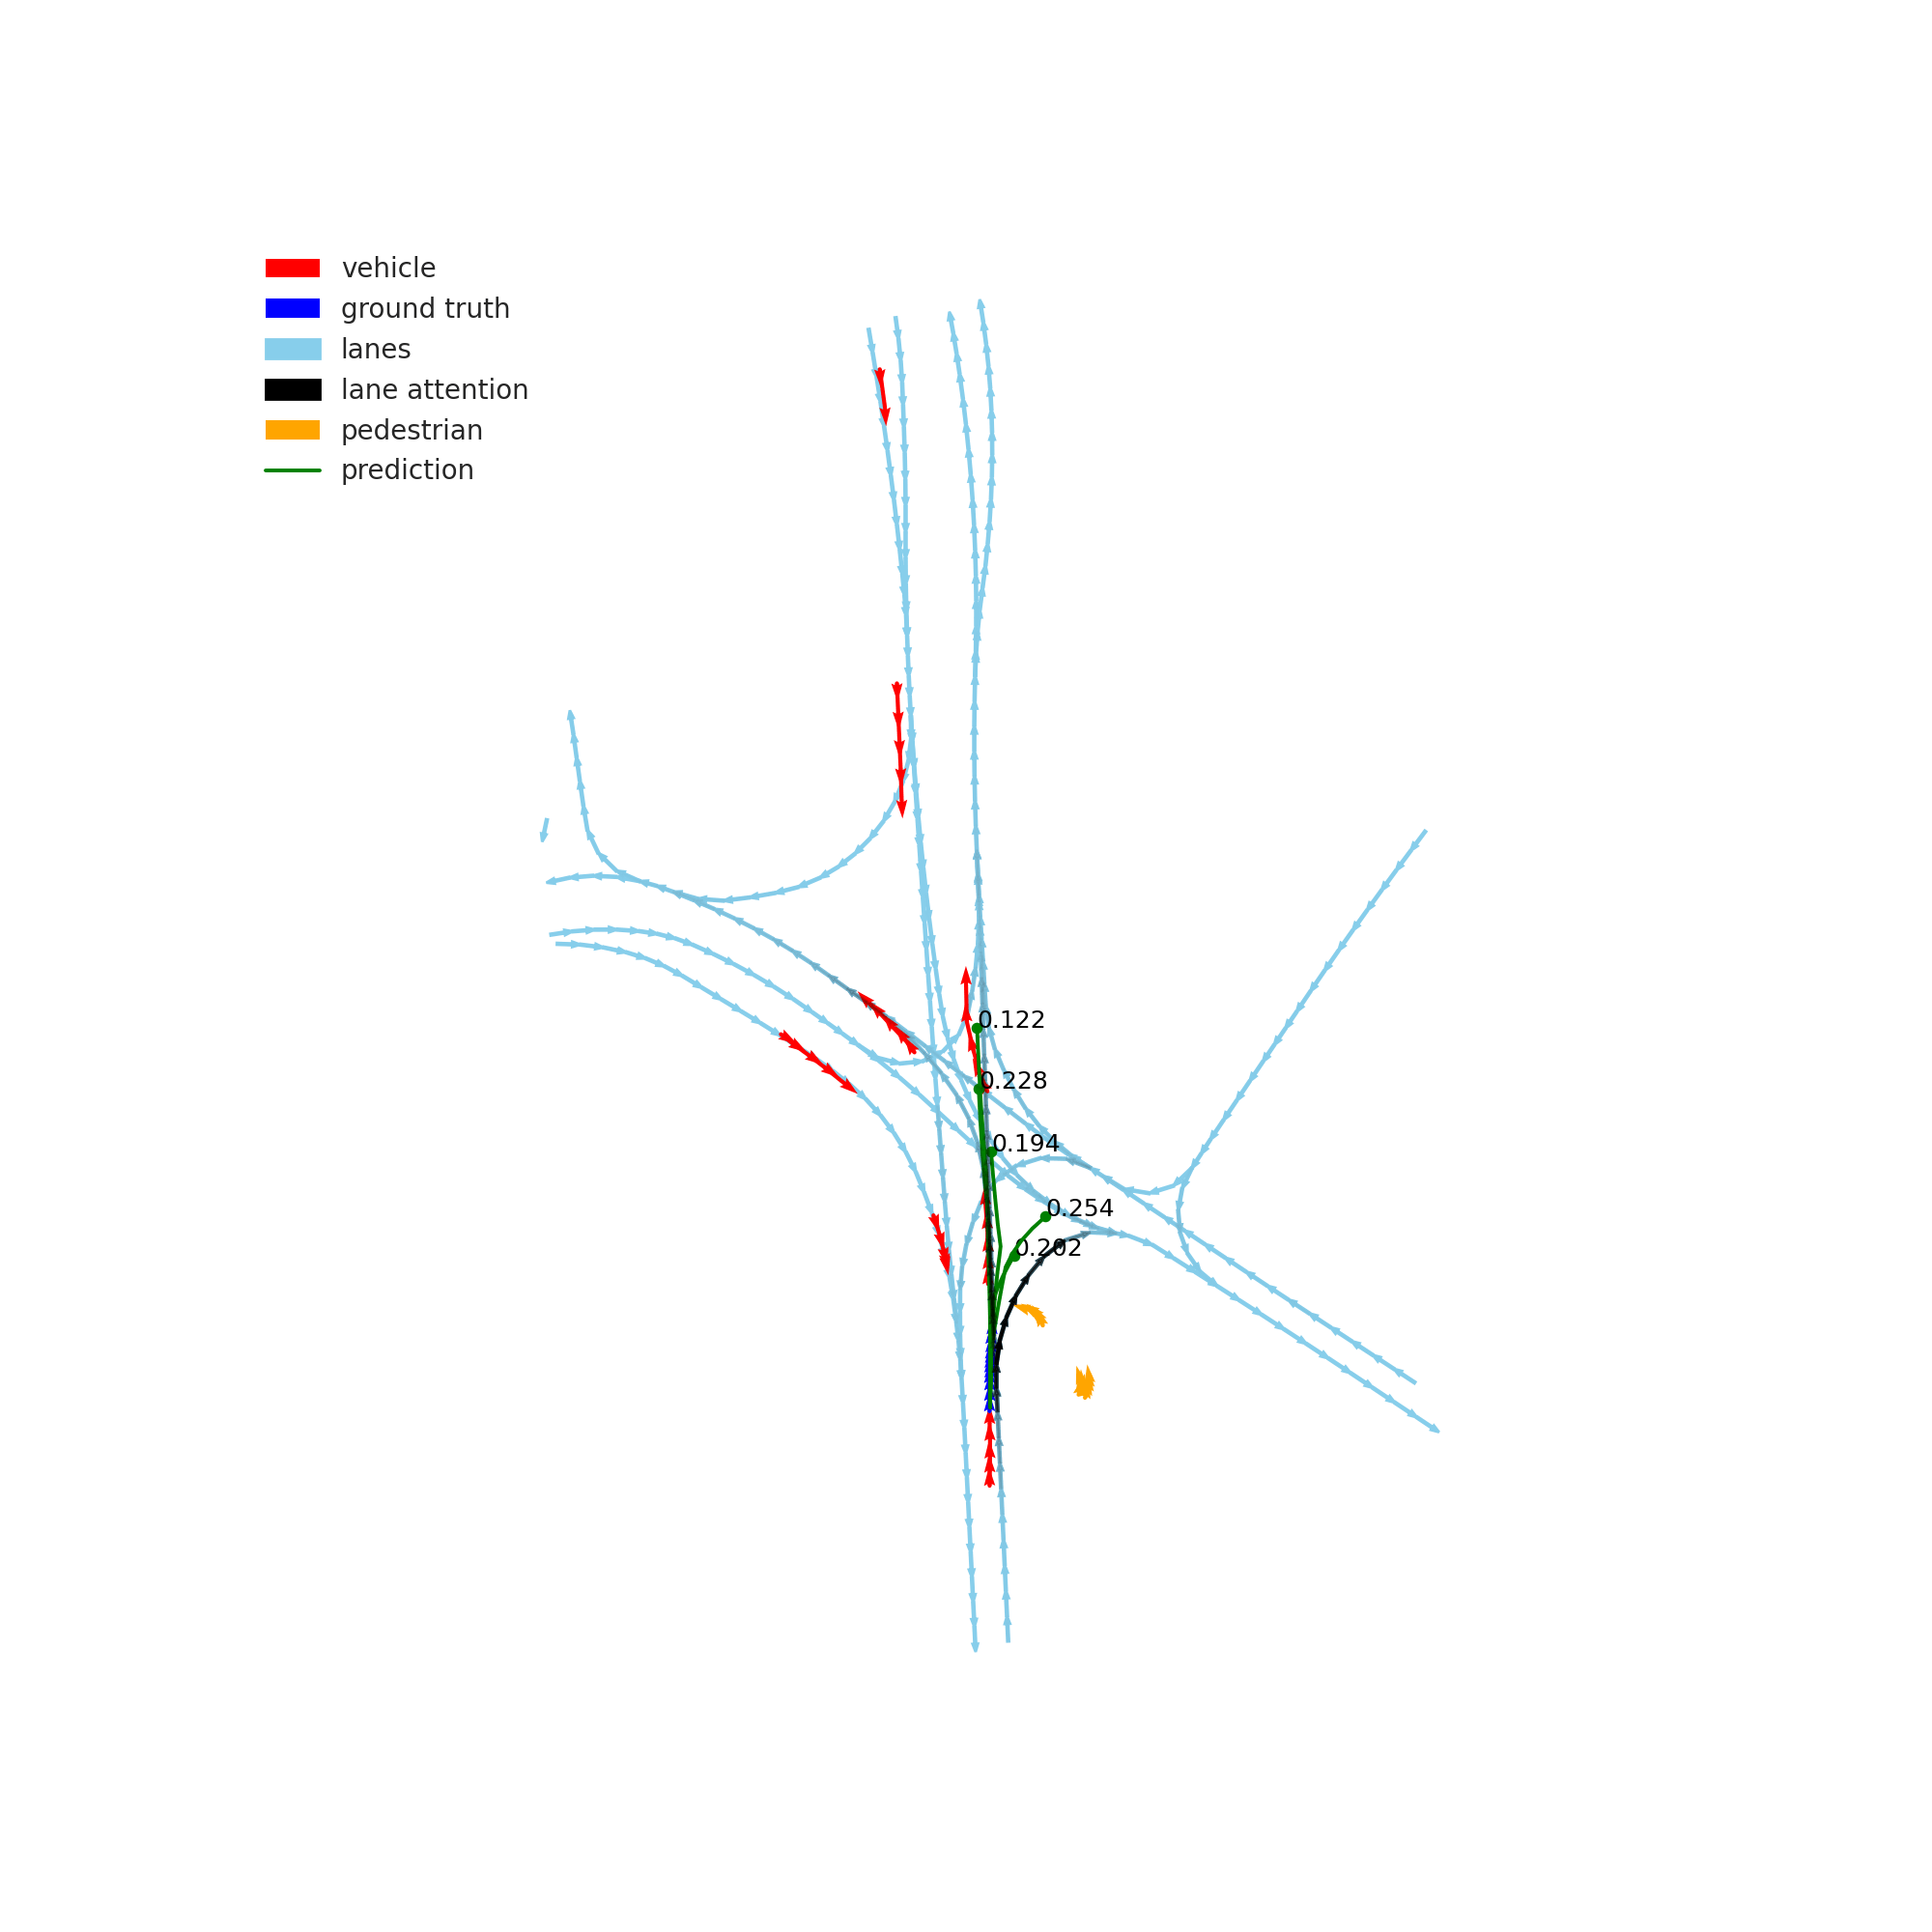
\includegraphics[width=0.2\linewidth,trim={110 500 450 85},clip]{images_results/2706cc4eb61844a1a5c7a5cb766ffc2e_37ab2d88d07846ef96d5227e9c5a15d7_minADE5_5.01_0-min.png}};
    % \end{tikzpicture}
    \caption{Visualization of predicted trajectories (green) for a target agent at an unseen intersection during training. The model, trained on the Deep Scenario dataset, refines its predictions progressively from (a) to (c), achieving better alignment with the lane structure. However, as shown in the second row, a limitation of our approach becomes evident: despite the attention maps indicating that the network should predict right-turn trajectories, it fails to generate them.}
    \label{fig:cross_data_qual}    
\end{figure}

\begin{table}[b]
    \centering
    \caption{LMFormer Cross Datataset performance validated on nuScenes validation split}
    \label{tab:train_ds_eval_nuScenes}
    \resizebox{\linewidth}{!}{
    \begin{tabular}{c c|c c c|c}
    \hline
    \multicolumn{2}{c|}{Training Dataset} & & & & \\
    Deep Scenario & nuScenes & minADE\textsubscript{5}$\downarrow$ & MR\textsubscript{5}$\downarrow$ & minFDE\textsubscript{5}$\downarrow$ & OffRoad$\downarrow$ \\
    \hline
    \checkmark & - & 1.54 & 0.57 & 2.86 & 0.02\\
    - & \checkmark & 1.13 & 0.48 & 2.13 & 0.01 \\
    \checkmark &\checkmark & 1.10 & 0.46 & 2.07 & 0.01\\
    \hline
    % \checkmark & - & 1.56 & 0.57 & 3.02 & 0.02 \\
    % - & \checkmark & 1.13 & 0.47 & 2.14 & 0.01 \\
    % \checkmark &\checkmark & 1.10 & 0.44 & 2.09 & 0.01\\
    \end{tabular}
    }
\end{table}

Furthermore, a quantitative evaluation of this model checkpoint, which is trained on Deep Scenario, is done on the nuScenes validation split to assess its cross-dataset generalization capabilities. The corresponding results are presented in Table \ref{tab:train_ds_eval_nuScenes}. It can be observed that the performance of this model checkpoint is significantly worse in comparison to the one trained on the nuScenes training set. In our analysis of this cross-dataset performance degradation, we identified a systematic underestimation of the predicted velocity in the case of Deep Scenario as compared to nuScenes. We attribute this discrepancy to the distributional differences between the datasets: Deep Scenario captures mainly slow-moving vehicles in intersection-heavy environments, while nuScenes provides a more diverse range of driving dynamics. To test this hypothesis, we train LMFormer on a combined dataset, containing training samples from both the nuScenes and Deep Scenario training sets. The corresponding qualitative results are shown in Table \ref{tab:train_ds_eval_nuScenes}. We observe that this model checkpoint outperforms the others trained individually on Deep Scenario and nuScenes training sets. This indicates that the network can learn to generalize better with more diverse datasets and can overcome limitations present in individual datasets, as previously reported in UniTraj \cite{feng2024unitraj}. It is important to note that the network architecture as well as the number of parameters were kept constant in the cross-dataset evaluations. 

In addition, we also illustrate the capability of LMFormer to predict multiple agents in parallel. Figure \ref{fig:scene_prediction} shows a marginal scene prediction output, where the trajectories are predicted in a single forward pass for all vehicles in the scene. 
\begin{figure}
    \centering
    \begin{subfigure}[t]{0.4\linewidth}
        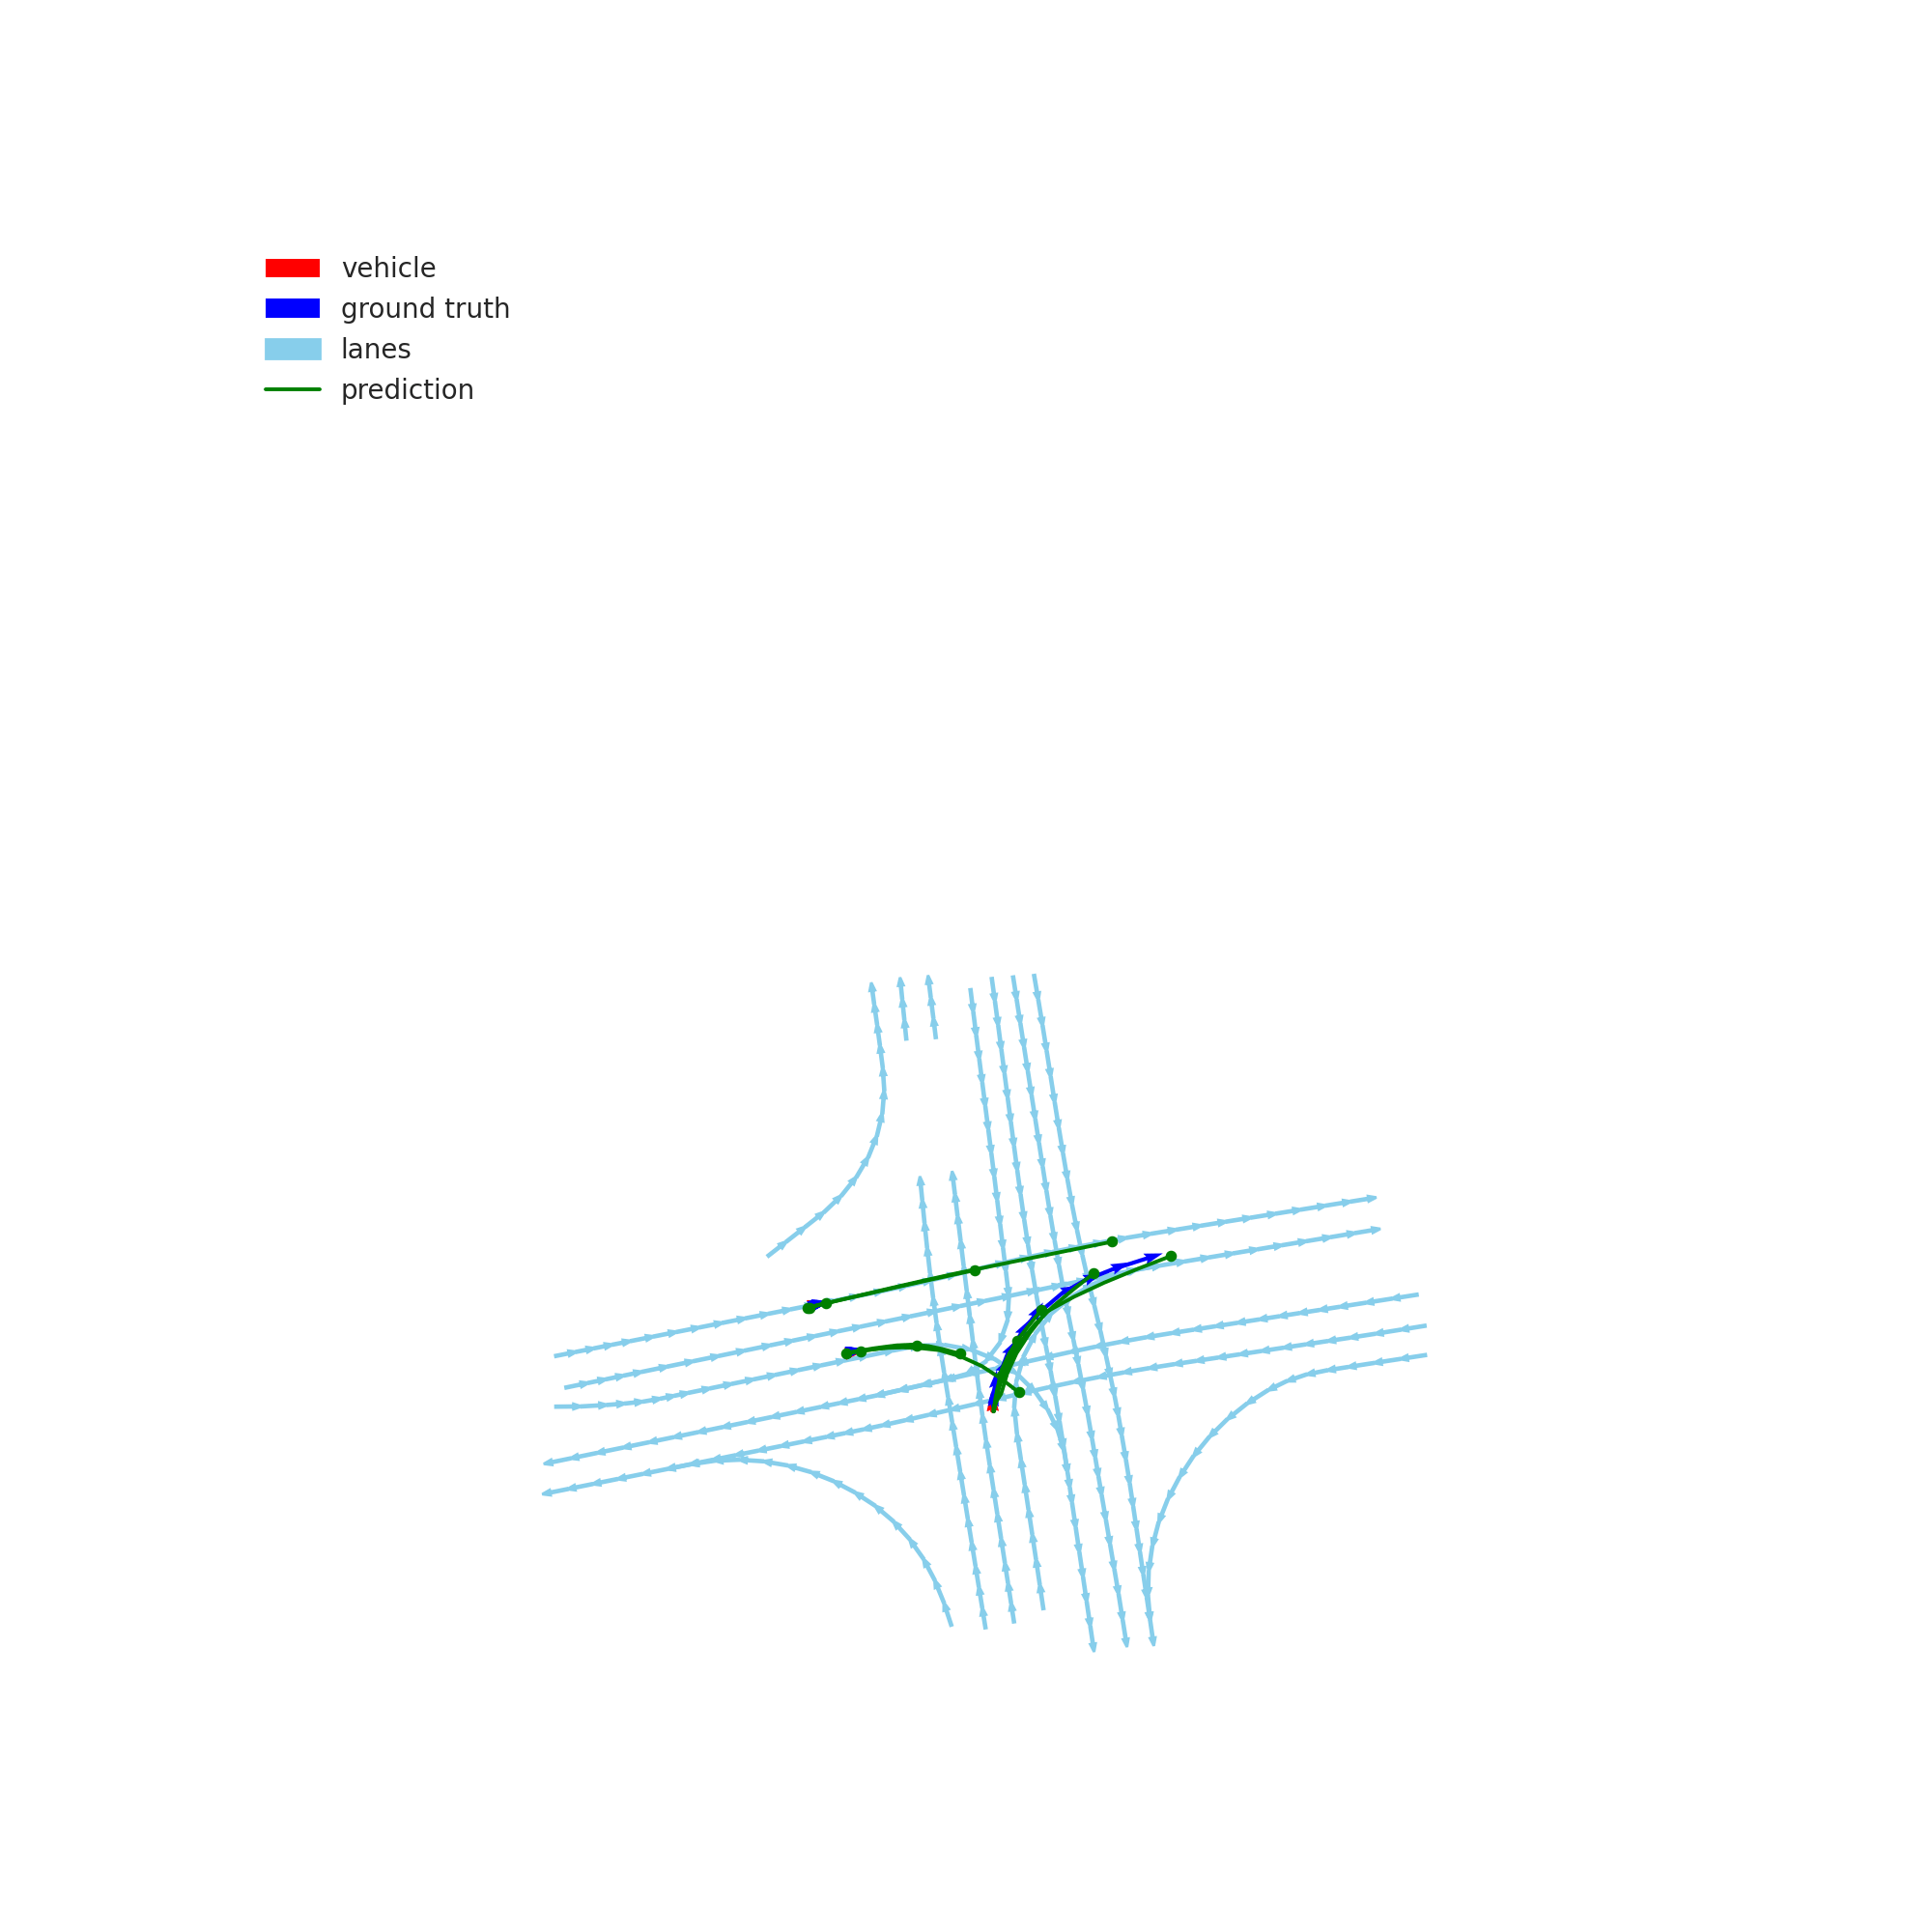
\includegraphics[height=4cm,trim={270 100 250 350},clip]{images_results/0044aaa230fe4cbeb4b744031e33af29_fb907b8b05644df28d64d6e25e9a956c_2-min.png}
        % \caption{Final Trajectories}
    \end{subfigure}
    \begin{subfigure}[t]{0.2\linewidth}
        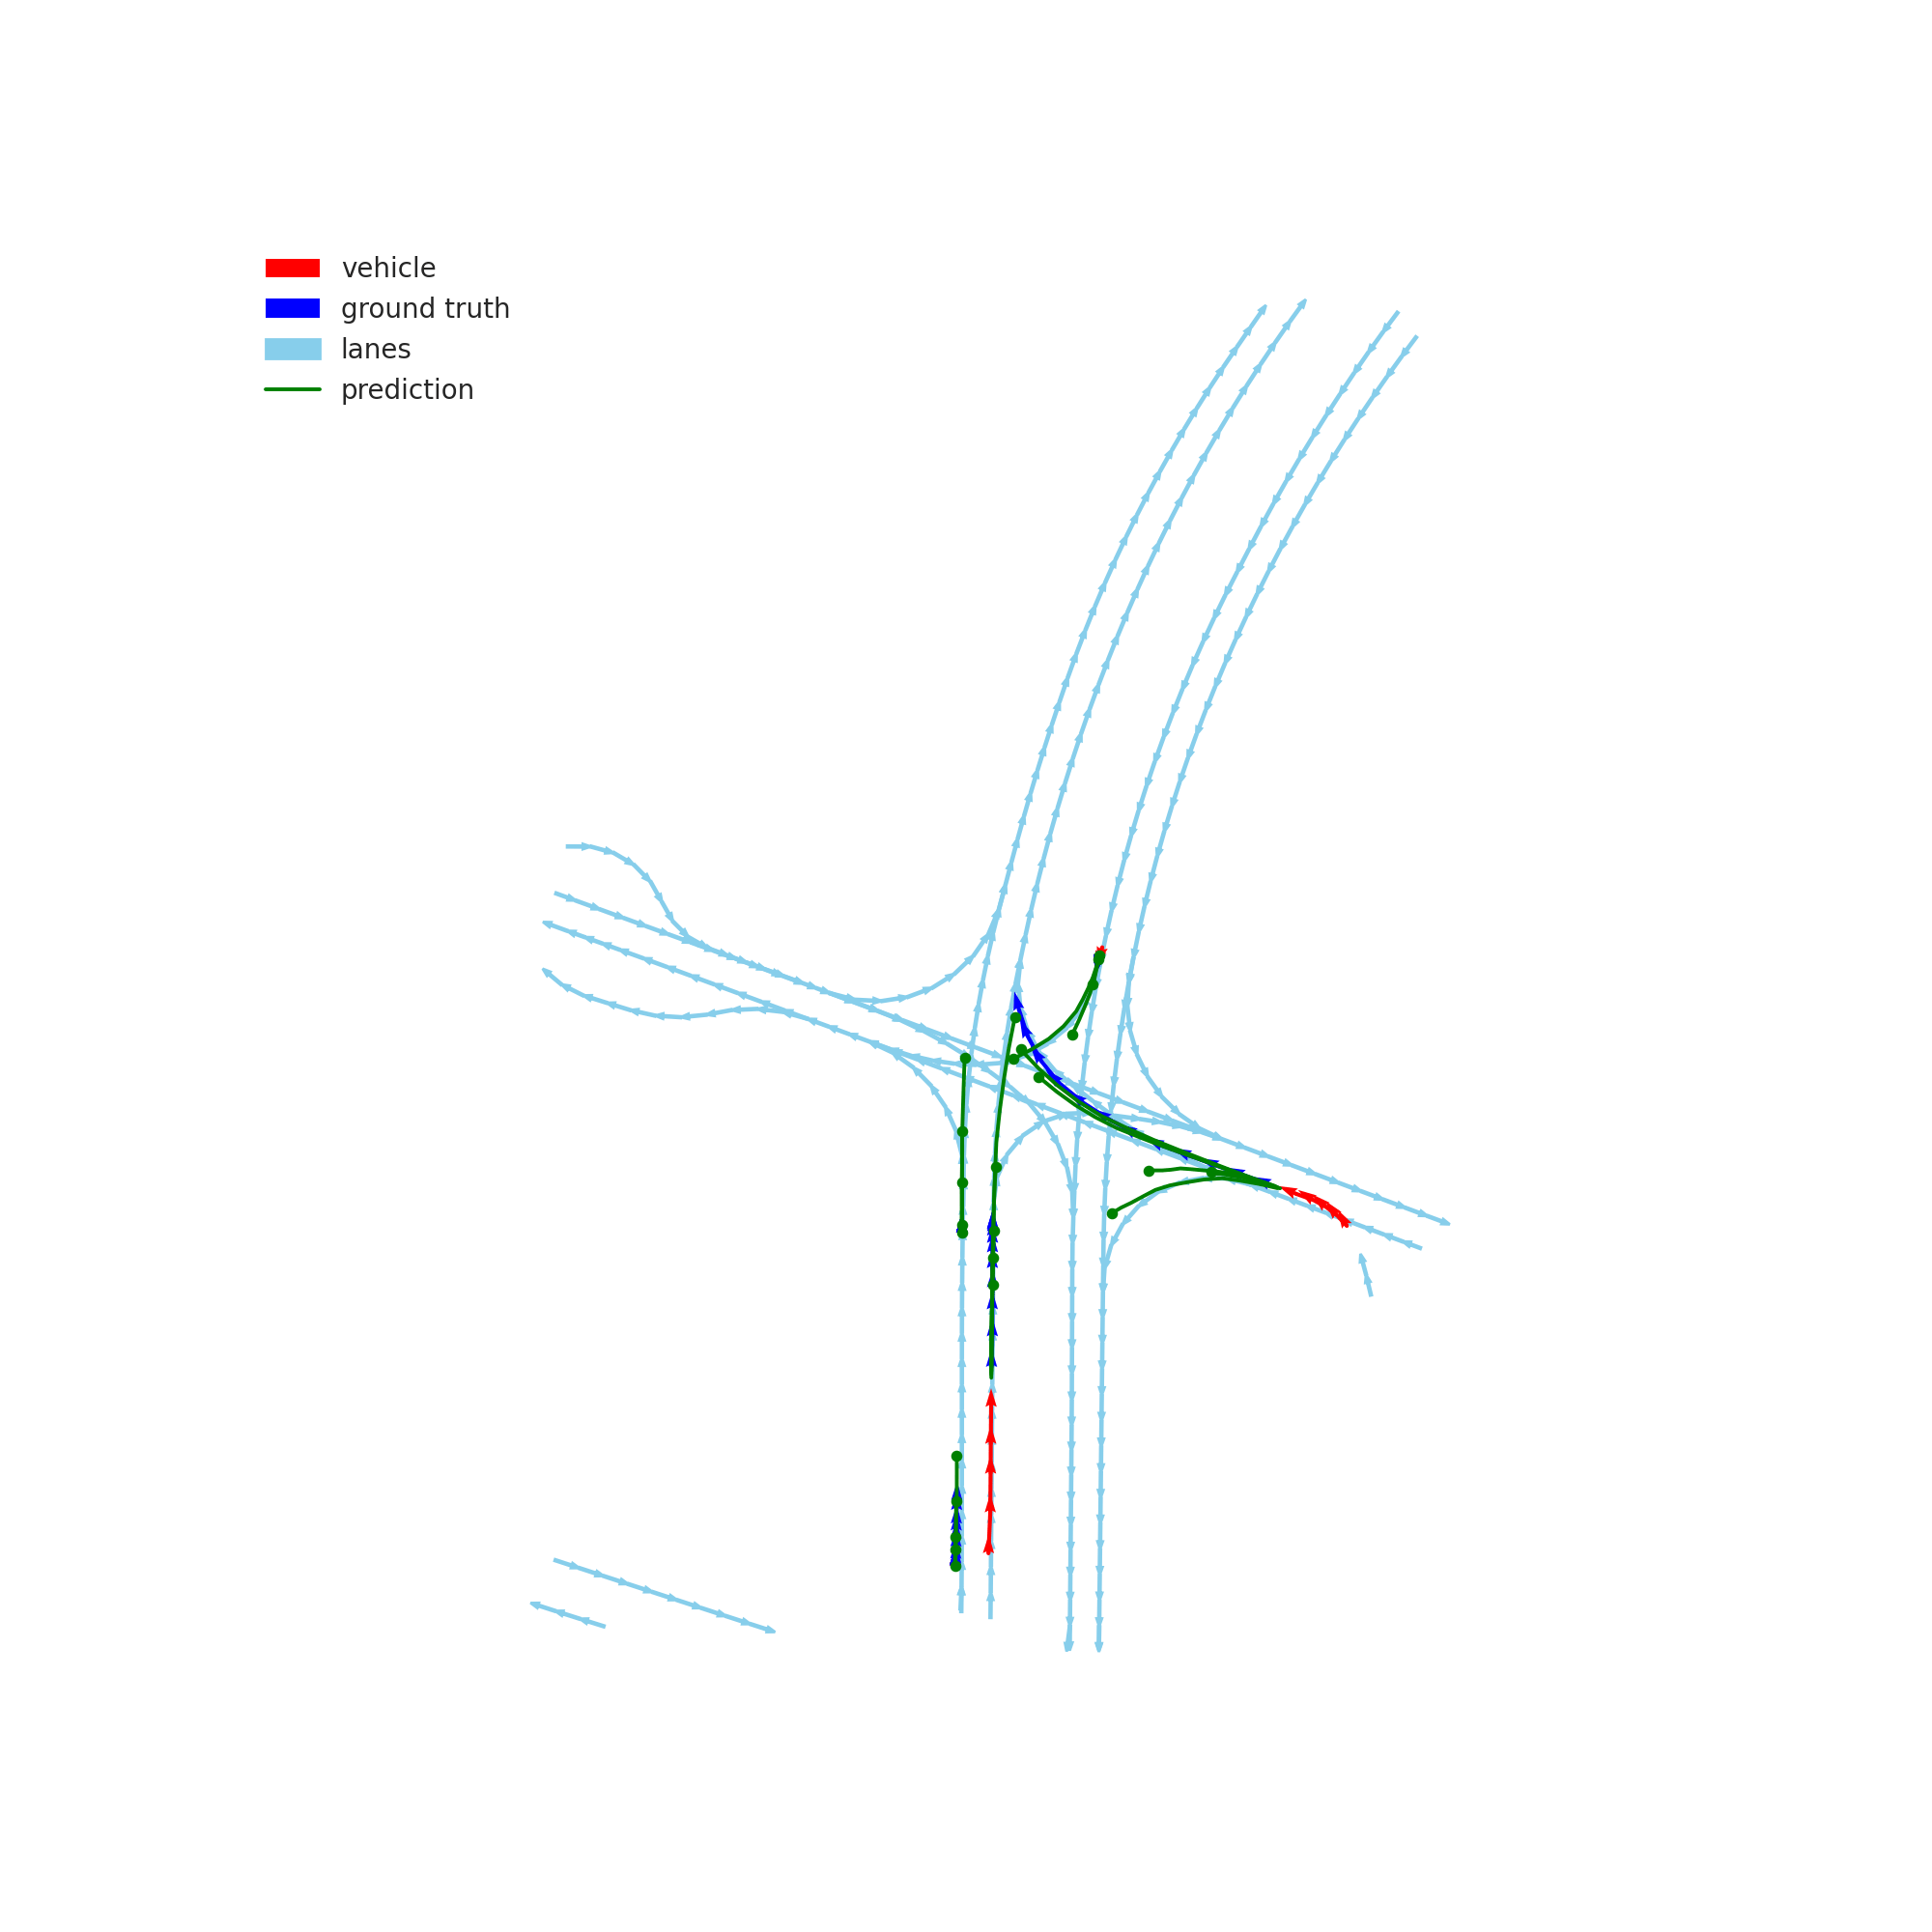
\includegraphics[height=4cm,trim={280 130 240 300},clip]{images_results/6c245e7d868c4be5a9c23c816701b103_c03d17123c6345f1a4626c6245b2c962_2-min.png}
        % \caption{Final Trajectories}
    \end{subfigure}
    % \begin{tikzpicture}[remember picture,overlay]
    %  \node at (0,7)      {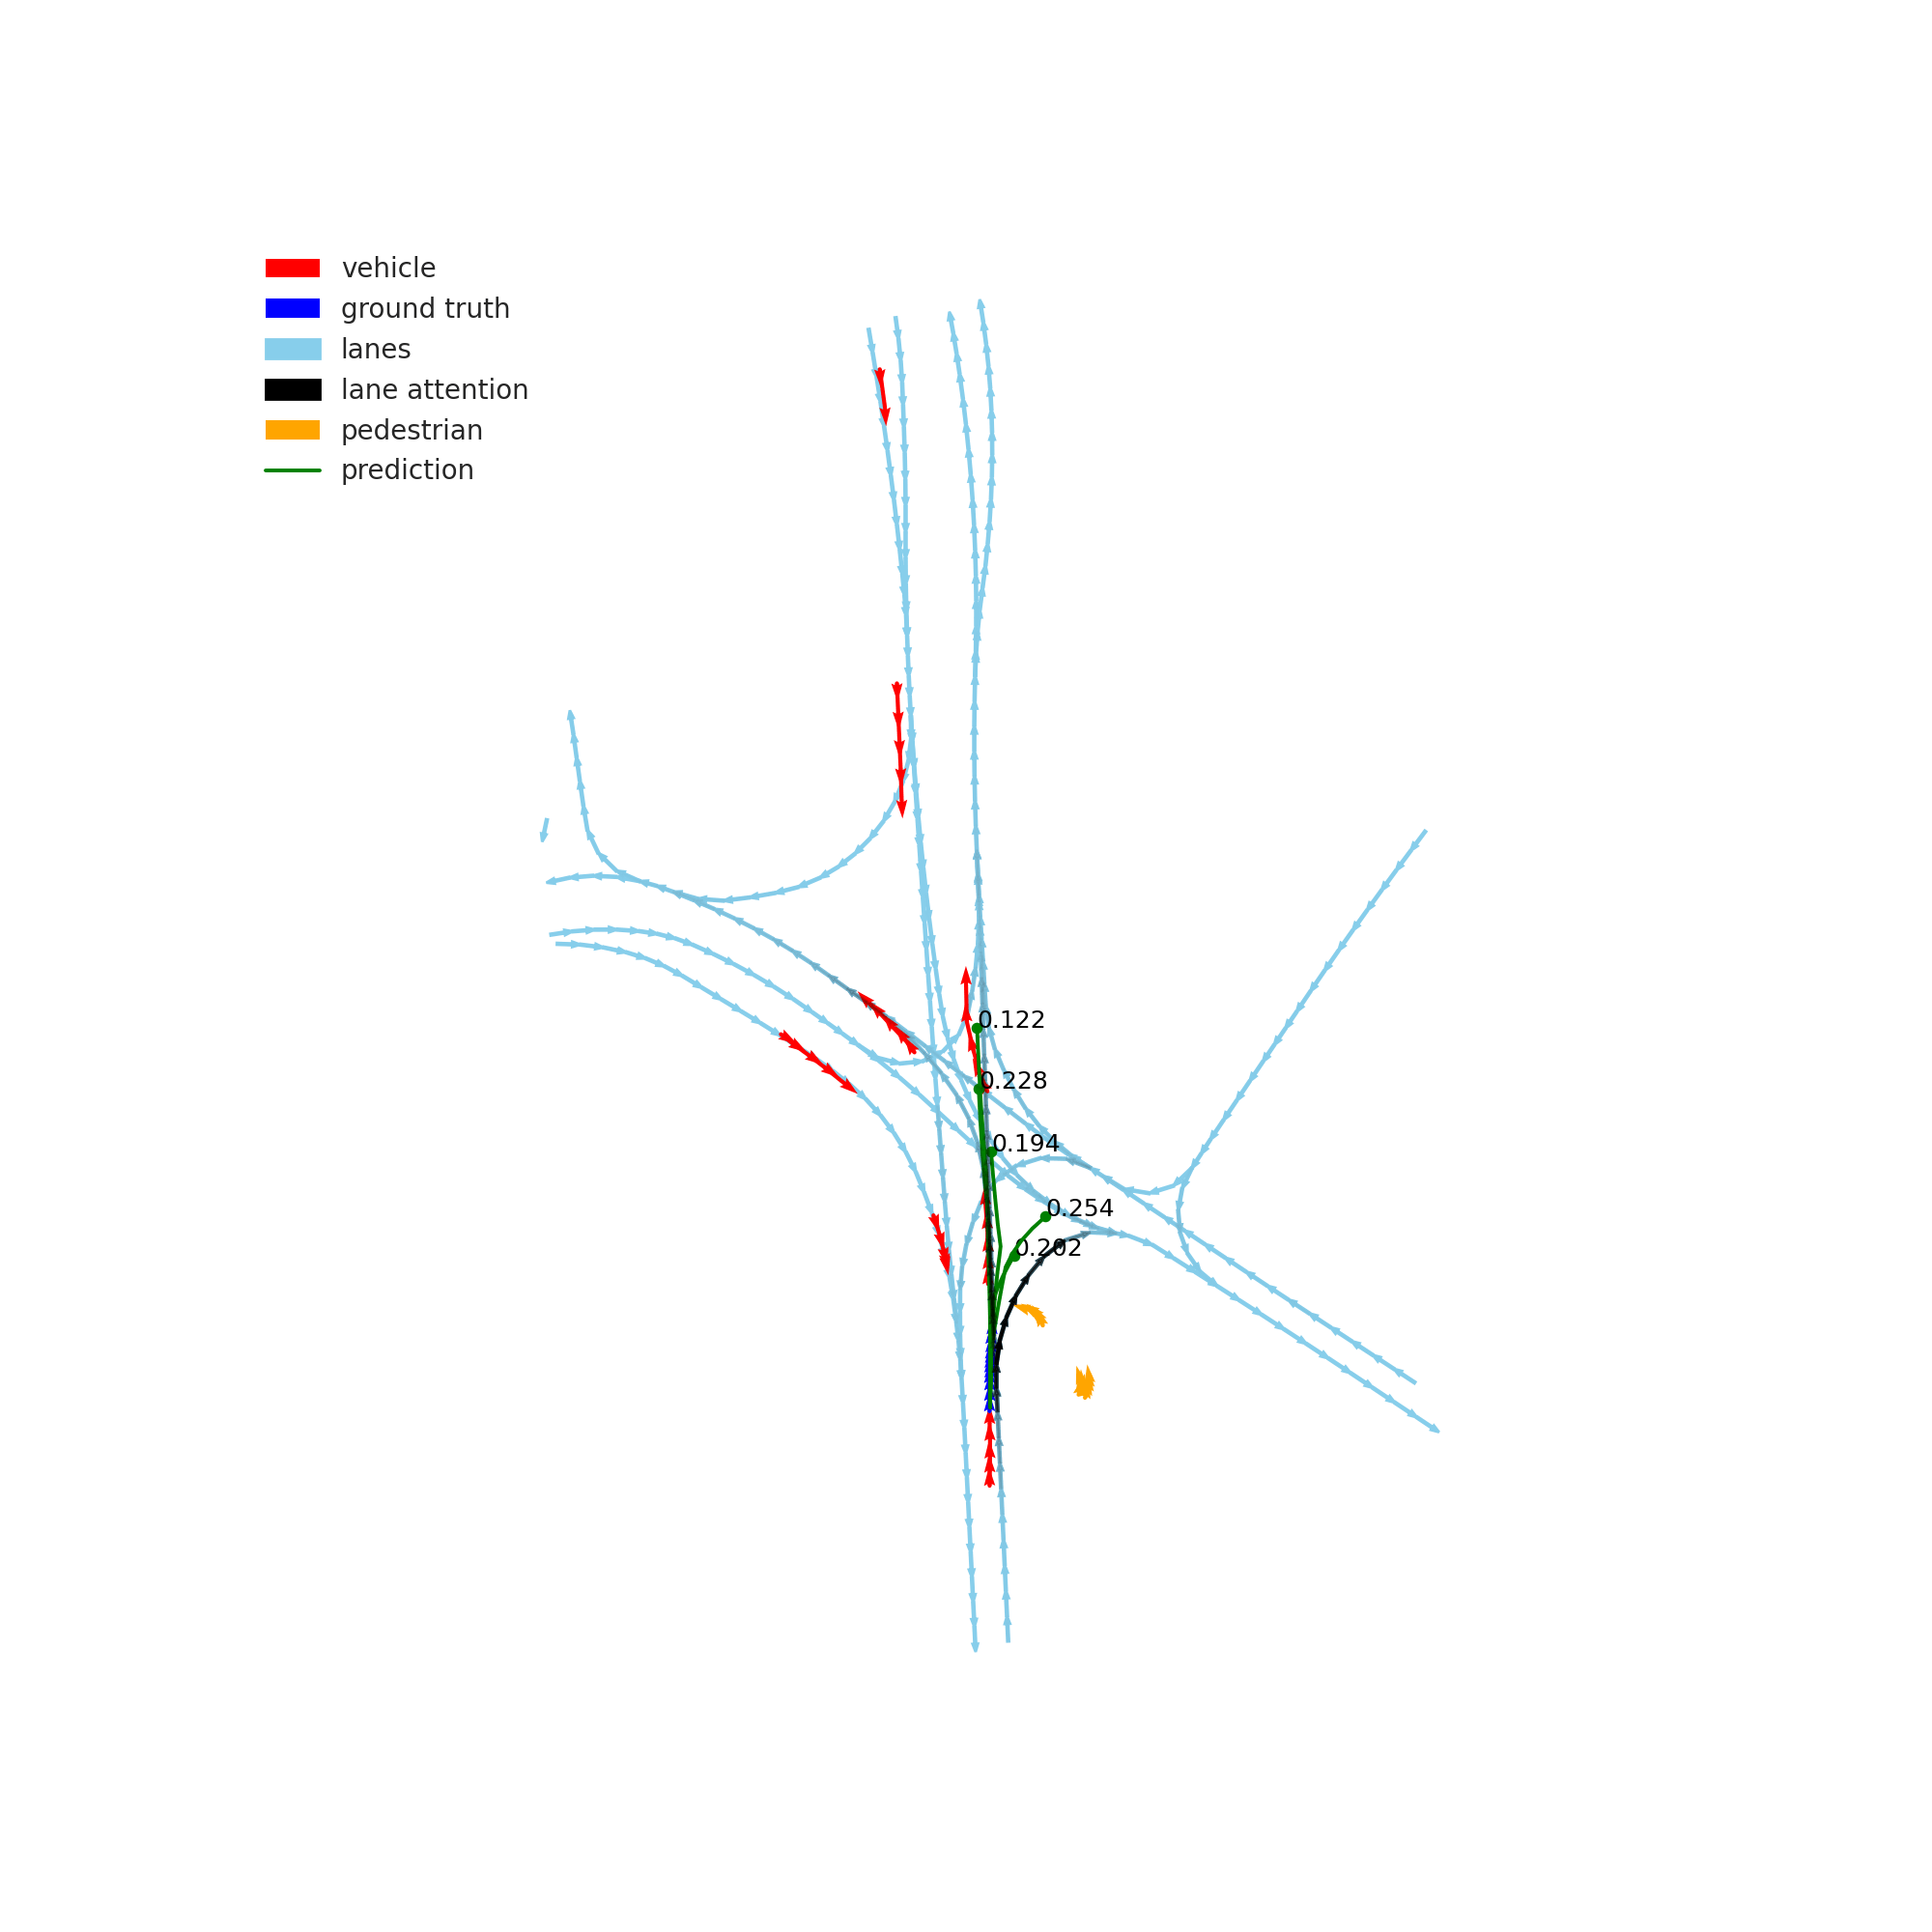
\includegraphics[width=0.2\linewidth,trim={110 500 450 30},clip]{images_results/2706cc4eb61844a1a5c7a5cb766ffc2e_37ab2d88d07846ef96d5227e9c5a15d7_minADE5_5.01_0-min.png}};
    % \end{tikzpicture}
    \caption{A depiction of marginal scene prediction. It illustrates the capability that LMFormer can be extended to multi-agent prediction.}
    \label{fig:scene_prediction}    
\end{figure}


\subsection{Ablations}\label{subsection:ablations}
In our ablation study, we validate the two key components of our approach: (1) the refinement strategy and (2) the long-range lane encoder. To evaluate the impact of refinement, we remove the additional regression loss introduced by the refinement layers. Similarly, we remove the lane self-attention module to evaluate the role of long-range lane interactions within the Map Encoder. The results of the ablation are presented in Table \ref{tab:ablation}. These results show that removing either component leads to a degradation in performance, with the degradation being slightly more pronounced when refinement losses are omitted. Overall, the ablation study confirms that both proposed components contribute significantly to SOTA performance.

\begin{table}[h]
    \centering
    \caption{Ablation Study conducted on the nuScenes val split}
    \label{tab:ablation}
    \resizebox{\linewidth}{!}{
    \begin{tabular}{c c|c c c|c}
    \hline
    \makecell{Lane \\ Self Attention} & Refinement & minADE\textsubscript{5}$\downarrow$ & MR\textsubscript{5}$\downarrow$ & minFDE\textsubscript{5}$\downarrow$ & OffRoad$\downarrow$ \\
    \hline
    \checkmark & \checkmark & 1.13 & 0.48 & 2.13 & 0.01 \\
     \checkmark & - & 1.16 & 0.51 & 2.20 & 0.01 \\
    - & \checkmark & 1.15 & 0.49 & 2.19 & 0.01 \\
    \hline
    %  \checkmark & \checkmark & 1.13 & 0.47 & 2.14 & 0.01 \\
    %  \checkmark & - & 1.14 & 0.48 & 2.16 & 0.01 \\
    %  \checkmark & - & 1.15 & 0.48 & 2.16 & 0.01 \\
    % - & \checkmark & 1.15 & 0.47 & 2.19 & 0.01 \\
    % - & \checkmark & 1.15 & 0.47 & 2.18 & 0.01 \\
    \end{tabular}
    }
\end{table}